% Arbeit.tex
% LaTeX-Hauptdatei fuer Studien/Diplomarbeiten am IMMD 9
% geschrieben von Wolfgang Heidrich <wgheidri@immd9.informatik.uni-erlangen.de>
% erweitert von Christian Vogelgsang <cnvogelg@immd9.informatik.uni-erlangen.de>
% benoetigt LaTeX 2e (z.B. in teTeX)

% --- Style + Optionen ---
% Font: 11pt bevorzugt, 10pt fuer besonders lange Arbeiten.
%       12pt nur in Ausnahmefaellen.
\documentclass[11pt, twoside, openright]{studdipl} 

% --- Paketauswahlt ---
% a4wide: breites Papierformat
% german: Deutsche Ueberschriften
% epsfig: figures mit EPS Bilder
\usepackage{a4wide,german}
\usepackage{graphicx}
\usepackage{color}

%%%%%%%%%%%%%%%%%%%%%%%%%%%%%%%%%%%%%%%%%%%%%%%%%%%%%%%%%%%%%%
%\usepackage[pdftex]{graphicx}
\DeclareGraphicsExtensions{.pdf,.png,.jpg}
\usepackage[german]{babel} %english language support
\usepackage[T1]{fontenc}
\usepackage{a4wide} % enlarges the A4 printing area
\usepackage{abbrevs} % defines abbreviation macros
\usepackage{amsmath} % mathematic formulas
\usepackage{amssymb} % mathematic special characters
\usepackage{dsfont}  % double stroke font (e.g. for mathematical sets)
\usepackage{ifthen}
\usepackage{float} % 3 different styles of float environments (tables or figures): plain, boxed and ruled
\usepackage{color} % displaying colors
\definecolor{mygray}{rgb}{0.5,.5,.5} % color define
\usepackage[absolute]{textpos} % absolute positioning of text
\usepackage[amssymb,thinqspace]{SIunits} % formatting support for the Systeme International d?Unites (SI)
\usepackage[printonlyused]{acronym} % management of acronyms and acronym lists (only used acronyms are printed in the list)
\usepackage{listings}  % embed listings (must be included before the package algorithm!
\usepackage{fancyhdr}% for funny headlines and footers
\usepackage{multirow} % tune tables
\usepackage[hang,small,bf]{caption} % smaller captions
\usepackage{vmargin} % pageaylout - borders
\usepackage{setspace} % Zeilenabst�nde..
\usepackage{titlesec} % formatting of sections etc.
\usepackage[colorlinks=true,
            citecolor=black,
            linkcolor=black,   % color of hyperref links
            urlcolor=black,       % color of page of \url{...}
            breaklinks=true    % break links if exceeding a single line
]{hyperref}
\usepackage[numbers]{natbib}
\usepackage{natbib}
\usepackage{engord} %english ordered numbers
\usepackage{soul}
\usepackage{captcont}

\pdfcompresslevel=0
\pdfoutput=1
\pdfcatalog{ /PageMode   /UseOutlines}

\usepackage[absolute]{textpos}
\usepackage{pdfpages}
\usepackage{csvsimple}


\newcommand{\citeeig}[1]{\citeauthor{#1} \cite{#1}}
\newcommand{\trade}{\textsuperscript{\textregistered}}
%%%%%%%%%%%%%%%%%%%%%%%%%%%%%%%%%%%%%%%%%%%%%%%%%%%%%%%%%%%%%%%%%%

% --- CV Config: ---

% --- weitere Pakete ---

% inputenc: direkte Eingabe von Umlauten erlaubt!
\usepackage[isolatin]{inputenc}
% huebsche Rahmen fuer Sourcecodebloecke
\usepackage{fancybox}
% erlaubt innerhalb eines Figure blocks mehrere Subfigures
\usepackage{subfig}  % urspruenglich subfigure
% verwende PostScript-Fonts
%\usepackage{pslatex}
\usepackage{times}
%\usepackage{dfadobe}           % ditto

% --- neue Environments ---

% \begin{cvSrcBox}.....\end{cvSrcBox} 
% Dies erzeugt eine Verbatim-Box mit einem Rahmen drumherum.
% Sie ist gut fuer Quelltextausschnitte geeignet!
\newenvironment{cvSrcBox}%
{\VerbatimEnvironment \begin{Sbox}\begin{minipage}{15cm}\begin{Verbatim}}%
{\end{Verbatim}\end{minipage}\end{Sbox}\setlength{\fboxsep}{3mm}\fbox{\TheSbox}}

% --- neue Kommandos ---

% \cvFig <file> <caption>
% Erzeugt eine Figure Umgebung mit einer xfig-Darstellung
% Die .fig Datei muss im Verzeichnis "figures" liegen
% Es wird automatisch ein Label mit dem Namen der Date erzeugt!
% Den Dateinamen ohne Endung .fig angeben!
\newcommand{\cvFig}[2]{\begin{figure}\begin{center}\input{figures/#1.tex}\end{center}\caption{\label{#1}#2}\end{figure}}

% \cvPic [width] <file> <caption>
% Erzeugt analog wie cvFig eine figure, doch diesmal mit einem
% Bild. Das Bild wird als PNG Datei in "pictures" abgelegt und
% dort automatisch nach EPS konvertiert.
\newcommand{\cvPic}[3][7cm]{\begin{figure}\begin{center}\includegraphics[width=#1]{pictures/#2.ps}\end{center}\caption{\label{#2}#3}\end{figure}}

% \cvPlot [width] <file> <caption>
% Erzeugt analog wie cvFig eine figure, doch diesmal mit einem
% Bild. Das Bild wird von GNUplot aus einer .plt-Datei erzeugt
\newcommand{\cvPlot}[3][10cm]{\begin{figure}\begin{center}\includegraphics[width=#1]{plots/#2.ps}\end{center}\caption{\label{#2}#3}\end{figure}}

% --- Optionen ---
% steuert das Figure Placement auf den Seiten
\renewcommand{\floatpagefraction}{0.8}

% definiert die Kopfzeile
\lhead[]{\fancyplain{}{\rightmark}}
\rhead[{\fancyplain{}{\leftmark}}]{}

% --- CV Config Ende ---

% Ein wenig liberalere spacing rules
\frenchspacing

% Erlaube groessere Freiraeume zwischen Woertern.
% (wichtig fuer Deutsche Texte wegen der grossen durchschnittlichen
% Wortlaenge). Fuer Englische Arbeiten moeglicherweise weglassen.
\sloppy

% -------------- Konfiguration ------------------------------------------------
% hier werden die individuellen Parameter der Arbeit festgelegt
% -> ALSO AENDERN!

% Typ der Arbeit auswaehlen:
%\thesistype{Studienarbeit}
\thesistype{Masterarbeit}

% Titel der Arbeit
\title{Farbnormalisierung f�r die automatische Klassifikation von Knochenmarkzellen}

% AutorIn <- Dein Name :-)
\author{Wolfgang Aichinger}

% Dein Geburtsdatum
\birthday{16. April 1991}

% Dein Geburtsort:
\birthplace{Deggendorf}

% DeinE BetreuerIn:
\supervisor{Dipl.-Inf. Sebastian Krappe}

% Beginn der Arbeit
\bdate{02. November 2015}

% Abgabetermin
\edate{02. Mai 2016}

% -------------- Ende der Konfiguration ---------------------------------------

\setcounter{secnumdepth}{3}
\setcounter{tocdepth}{5}

\begin{document}

% DRAFT MODE
% Erzeugt eine Ueberschrift mit dem Datum des Drafts. Muss fuer die
% endgueltige Version natuerlich auskommentiert werden!!!
%\draft

% Der "Vorspann" hat roemische Seitennummern 
\prepages

% Damit wird die zweite Titelseite erstellt (die erste ist ja in einem
% separaten File)
\maketitle

% eine Leerseite
\vspace*{10cm} \newpage

% Inhaltsverzeichnis
\tableofcontents\newpage
% Verzeichnis aller Zeichnungen - optional
\listoffigures\newpage
% Verzeichnis aller Tabellen - optional
\listoftables\newpage

% eine Leerseite
\vspace*{10cm} \newpage

% der eigentliche Text hat arabische Nummern
\mainbody

% sorgt dafuer, dass alle Eintraege der Literature.bib im 
% Literaturverzeichnis aufgefuehrt werden
\nocite{*}

% ---------- Kapitel ---------
% Die Datei Chapter.tex wird automatisch erzeugt!

%\setlength{\parskip}{-0.5ex plus1ex}

\newpage
\pagenumbering{arabic}
\pagestyle{fancy}
\chapter[Einleitung]{Einleitung}\label{sec:einleitung}
%\begin{tikzpicture} 
%	\begin{axis}[ 
%		xlabel=Bild, 
%		ylabel=Metrik,
%	 	axis x line*=bottom,
%	 	axis y line*=left,
%	 	ymajorgrids,
%	 	ymin=0,
%	 	ymax=1
%	] 
%	 \addplot [
%	 	color=blue,
%       ultra thick,
%      point meta=x, % Define the value that's used to determine the color
%        mark=x
%    ] coordinates { 
%	(1, 1) 
%	(2, 0.689128518) 
%	(3, 0.313492749)
%	(4, 0.197890621)
%	(5, 0.155663954)
%	(6, 0.135560304)
%	(7, 0.125045233)
%	(8, 0.119600855)
%	(9, 0.114321953)
%	(10, 0.112258035)
%	}; 
%	\end{axis} 
%\end{tikzpicture}



\section[Motivation]{Motivation}\label{sec:motivation}
Knochenmarkanalysen werden im klinischen Alltag in den verschiedensten F�llen angefordert, z.B. bei Verdacht auf Leuk�mie, da es sich hierbei um eine Erkrankung des Knochenmarks handelt. Die Krankheit kann in allen Altersgruppen auftreten, es wird zwischen den folgenden, h�ufigsten, Formen je nach Verlauf und urs�chlichem Zelltyp unterschieden:
\begin{itemize}
\item{Akute myeloische Leuk�mie (AML)}
\item{Chronische myeloische Leuk�mie (CML)}
\item{Akute lymphatische Leuk�mie (ALL)}
\item{Chronische lymphatische Leuk�mie (CLL)}
\end{itemize}
Im Kindesalter tritt fast immer ein akuter Verlauf auf, am h�ufigsten wird eine ALL diagnostiziert. Unabh�ngig vom Alter bildet jedoch die CLL mit �ber einem Drittel die zahlreichste Form. Im Jahr 2012 lag die Zahl der Neuerkrankungen an Leuk�mie bei ca. 12640 F�llen, 5\% davon unter 15 Jahren. Eine �bersicht �ber das Alter der neuerkrankten Patienten zeigt Abbildung \ref{fig:leukemia_age}. Aus dieser Statistik geht ebenfalls hervor, dass vor allem im Erwachsenenalter M�nner h�ufiger betroffen sind als Frauen.
\begin{figure}
\center
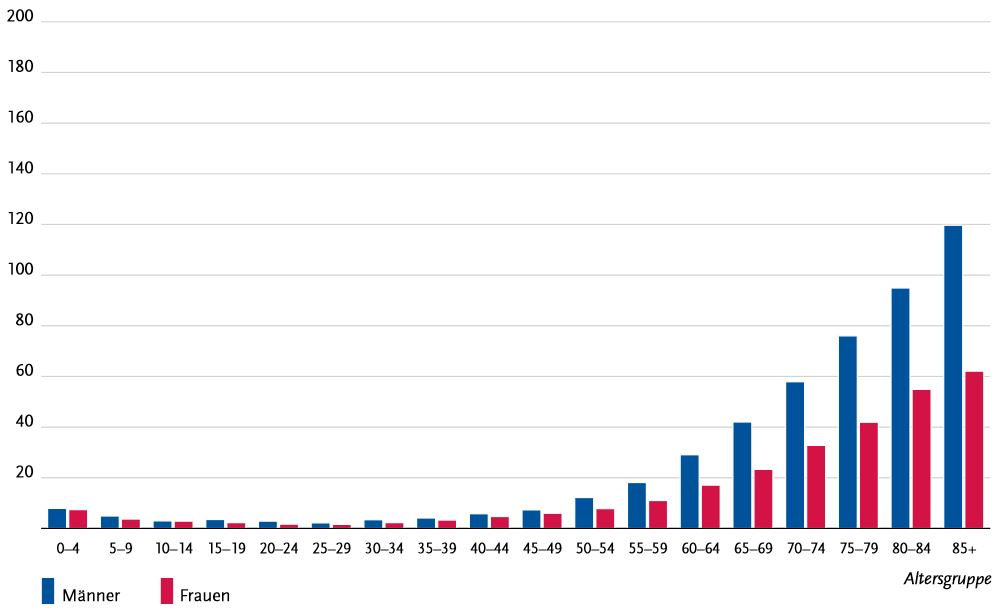
\includegraphics[width = 0.9\textwidth]{pics/Einleitung/leukaemie_statistic_age}
\caption[Neuerkrankungen Leuk�mie nach Alter und Geschlecht]{Die Graphik zeigt die Statistik der Neuerkrankungen mit Leuk�mie in Deutschland f�r die Jahre 2011 und 2012 nach Alter (horizontale Achse) und Geschlecht (Balkenfarbe). Die Zahlen sind dabei relativ je 100.000 normiert \cite{url_leukemia_statistic}.\label{fig:leukemia_age}}
\end{figure}
Bei Kindern ist die Prognose deutlich g�nstiger als bei Erwachsenen. Die 5-Jahres �berlebenschance wird f�r sie mit bis zu 90\% angegeben, der Wert f�r die Erwachsenen liegt nur bei 35-50\%. Eine dauerhafte Heilung ist m�glich, es gibt sie aber nur selten z.B. durch Stammzellentransplantation. �ber die Ursachen von Leuk�mie ist indes wenig bekannt. Als Risikofaktoren gelten ionisierende Strahlung, z.B. bei Strahlen- oder Chemotherapie, und der Umgang mit Chemikalien wie Benzol. Diese Faktoren treffen aber nur auf eine kleine Gruppe der Erkrankten zu, weshalb weitere Faktoren diskutiert werden, ohne dass diese bis jetzt nachgewiesen werden konnten. Hierzu geh�ren Ern�hrungsgewohnheiten und Lebensstil, vor allem beim chronischen Verlauf, ein Einfluss von Viren und ein ungen�gendes Training des Immunsystem bei Heranwachsenden \cite{url_leukemia_statistic}.
Eine Leuk�mie macht sich in Proben des Knochenmarks dadurch bemerkbar, dass die Leukozytenzahl zugunsten anderer Zelltypen deutlich zunimmt, was Blutarmut und Probleme bei der Gerinnung zur Folge haben kann. F�r den Nachweis muss daher eine repr�sentative Anzahl an Zellen einer Klasse zugeordnet und gez�hlt werden. Dieser Vorgang ist zeitaufwendig und nicht standardisiert, weshalb es zu Abweichungen bei der Analyse durch verschiedene H�matologen kommen kann. Bei der wiederholten Auswertung durch den gleichen Arzt treten ebenfalls Diskrepanzen auf.
Das Ziel eines Projekts am Fraunhofer-Institut f�r Integrierte Schaltungen IIS ist es deshalb, den Prozess der Differentialz�hlung zu automatisieren, wodurch Ressourcen gespart werden k�nnen und eine bessere Vergleichbarkeit erzielt wird. Hierzu wurden Algorithmen entwickelt, um Zellen in gef�rbten Ausstrichen zu detektieren, zu segmentieren und zu klassifizieren. Diese Aufgabe wird dadurch erschwert, dass die Pr�parierung zwar Standards unterliegt, sich das Erscheinungsbild aber abh�ngig von Probendicke, Farbmenge, verwendetem Mikroskop usw. unterscheidet.
 
\section[Aufgabenstellung]{Aufgabenstellung}\label{sec:aufgabenstellung}
Das Ziel der vorliegenden Arbeit ist es, verschiedene Ans�tze zur Farbnormalisierung zu entwickeln, zu implementieren und miteinander zu vergleichen. Zun�chst soll hierf�r eine Literaturrecherche �ber g�ngige Verfahren sowie deren Eignung f�r das vorliegende Problem durchgef�hrt werden. Bestehende Verfahren sollen umgesetzt und gegebenenfalls angepasst und erweitert werden. Der Fokus der Evaluierung liegt auf dem Einfluss auf die Qualit�t der vorhandenen Segmentierungs- und Klassifikationsalgorithmen f�r Knochenmarkzellen. 

\chapter[Allgemeine Grundlagen]{Allgemeine Grundlagen}\label{sec:grundlagen}

\section[Mikroskopie]{Mikroskopie}\label{sec:mikroskopie}
F�r die Pathologie und H�matologie spielt das Lichtmikroskop eine entscheidende Rolle. Mit Hilfe der optischen Vergr��erung k�nnen Strukturen auf zellul�rer Ebene sichtbar gemacht werden, was diagnostische Aussagen erm�glicht. Grunds�tzlich besteht ein Lichtmikroskop aus Objektiv und Okular, wobei letzteres einer Lupe entspricht. Zun�chst wird durch das Objektiv ein virtuelles Zwischenbild erzeugt, welches dann durch das Okular wiederum gedreht und auf die Kameraebene projiziert wird \citep[6f]{haus2014optische}. Der schematische Aufbau eines solchen Ger�ts ist in Abb. \ref{fig:strahlengang} gezeigt.
\begin{figure}
\center
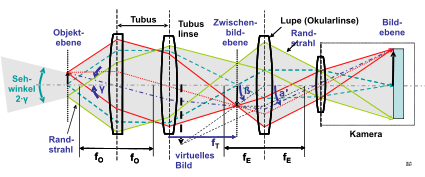
\includegraphics[width = 0.7\textwidth]{pics/Grundlagen/Mikroskop_Strahlengang}
\caption[Schematischer Strahlengang Mikroskop]{Strahlengang im Mikroskop: Weg von Strahlen aus der Objektebene durch den Tubus und die Okularlinse in die Bildebene \cite{url_mikroskop_strahlengang}.\label{fig:strahlengang}}
\end{figure}
Die gesamte Vergr��erung $M_{ges}$ ergibt sich durch Multiplikation der Teilvergr��erungen der beiden Komponenten, wie in Formel \ref{equ:zoom} angegeben. $\beta_{Obj}$ entspricht dabei dem Abbildungsverh�ltnis des Objektiv, z.B. "40:1", und $M_{Ok}$.
\begin{equation}\label{equ:zoom}
M_{ges} = \beta_{Obj}M_{Ok}
\end{equation}

Das Pr�parat ist in der Regel zun�chst nicht homogen ausgeleuchtet, wodurch eine sp�tere Analyse erschwert wird. Deshalb ist ein wichtiger Schritt beim Mikroskopieren das sogenannte K�hlern, wodurch Streulicht unterdr�ckt wird und die Beleuchtungsintensit�t auf ein relevantes Ma� reduziert wird. Hierdurch k�nnen auch licht- und w�rmeempfindliche Proben geschont werden \citep[19f]{haus2014optische}.    

\section[Knochenmarkdiagnostik]{Knochenmarkdiagnostik}\label{sec:diagnostik}
Das Knochenmark ist im menschlichen K�rper ab dem 4.-5. Schwangerschaftsmonat zust�ndig f�r  f�r die H�matopoese, also die Blutbildung. Zuvor �bernehmen diese Aufgabe der Dottersack (bis zur 6. Woche) und Leber und Milz(ab Woche zw�lf bis drei Wochen nach der Geburt). Bis zur Pubert�t sind fast alle Knochen beteiligt, ab dem 30 Lebensjahr dagegen nur noch kurze und platte Knochen. Hierzu z�hlen Beckenschaufel, Wirbelk�rper, Sternum, Rippen und der Sch�del. Ist der Bedarf erh�ht oder liegen knochenmarksverdr�ngende Prozesse vor, so k�nnen Milz, Leber und auch andere Organe f�r die H�matopoese reaktiviert werden. Aus einer multipotenten Stammzelle entstehen �ber mehrere Zwischenstadien die verschiedenen Zellarten \ref{fig:haematopoese}.
\begin{figure}
\center
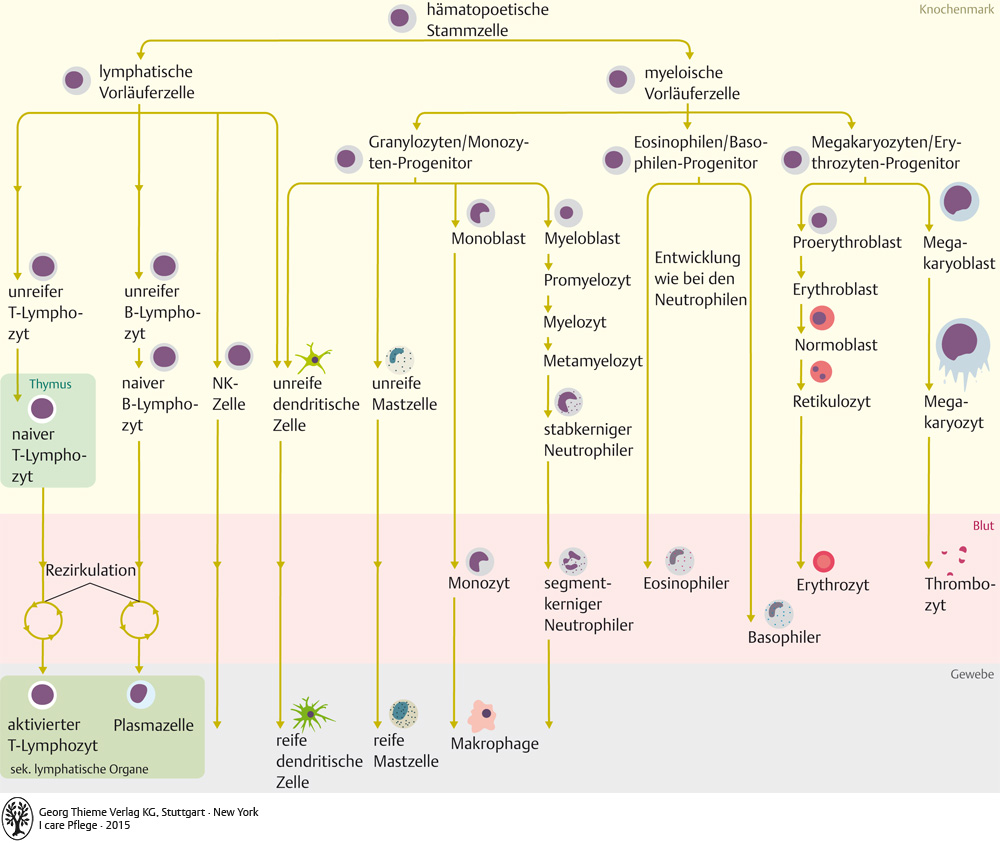
\includegraphics[width = 0.9\textwidth]{pics/Grundlagen/haematopoese}
\caption[Schema H�matopoese]{Die Abbildung zeigt die Entwicklung einer Stammzelle �ber Zwischenstadien zur fertigen Zelle\cite{url_haematopoese}\label{fig:haematopoese}}
\end{figure}  

Die Gr�nde f�r eine zytologische Untersuchung des Knochenmarks sind vielf�ltig und reichen von au�erhalb der Norm liegenden Differentialblutausstrichen bis zum Verdacht auf \leukaemie. Beim konventionellen Vorgehen wird zun�chst mit einer Punktionsnadel eine geringe Menge an Knochenmark entnommen. F�r die weitere Bearbeitung wird die Probe mit einer gerinnungshemmenden L�sung vermischt und auf einem Objekttr�ger ausgestrichen. Im Anschluss muss die Schicht eine Stunde trocknen und wird dann mit dem Verfahren nach Pappenheim gef�rbt, die eine Kombination aus zwei verschiedenen Methoden darstellt. Bei May-Gr�nwald kommt eine Eosin-Methylenblau-L�sung zum Einsatz, bei Giemsa dagegen Azur-Eosin-Methylenblau-L�sung, wobei Azur-Eosin eine Abwandlung zu Eosin darstellt. Diese Aufgabe �bernimmt ein Automat, der daf�r ca. 45 Minuten ben�tigt. Das Methylenblau ist positiv geladen und f�rbt somit negativ geladene Zellbestandteile. Die Ladung von gel�stem Eosin ist negativ, wodurch vor allem positive Proteinstrukturen der Zelle gef�rbt werden. Als Stabilisator dient indes Glycerin und als Fixiermittel wird Methanol verwendet\cite{fuchs2011manual}. 

Die Analyse der Probe findet unter einem Lichtmikroskop statt. Bei zehnfacher Vergr��erung kann dabei zun�chst eine Aussage �ber Zelldichte und Fettgehalt getroffen werden. Teilweise gibt es auf dieser Stufe auch schon Informationen �ber qualitative Ver�nderungen, z.B. H�ufung bestimmter Zelltypen. Geeignete Bereiche des Ausstrich werden anschlie�end bei st�rkerer Vergr��erung (63x, seltener auch 100x) quantitativ ausgewertet. Daf�r werden die verschiedenen Zelltypen gez�hlt, wobei mindestens 200 Zellen ausgewertet werden sollten, um Aussagen treffen zu k�nnen. Diese manuelle Auswertung dauert in der Regel zwischen 5 und 15 Minuten, in Einzelf�llen sogar bis zu 30 Minuten. Das Ergebnis dieser Differentialz�hlung ist entscheidend f�r das weitere diagnostische und therapeutische Vorgehen. Hat ein Patient z.B. \leukaemie, so wird dieses Verfahren eine deutlich erh�hte Leukozytenzahl aufdecken, welche die restliche Blutbildung verdr�ngt. \color{red}Quelle fehlt noch!\color{black}.
%TODO Quelle, Sebastian fragen!

\section{Bspline}\label{sec:basic_bspline}
Das Konzept der Bsplines erlaubt es Kurven zu modellieren, die ein Set von Kontrollpunkten mittels Teilpolynomen so ann�hert, dass sie an den Grenzen stetig sind. Der Grad der Stetigkeit ist dabei �ber den Grad des Bsplines $n$ festgesetzt. Die Kurve ist neben den Kontrollpunkten auch noch vom Knotenvektor $\mathbf{T} =  (t_i)$ beeinflusst, welcher die Parameterintervalle festlegt. Ein Beispiel eines Knotenvektors ist in Abbildung \ref{fig:knotvector} dargestellt.
\begin{figure}[h]
\center
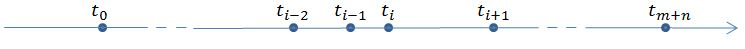
\includegraphics[width = 0.7\textwidth]
{pics/StandTechnik/knotvector}
\caption[Bspline Knotenvektor]{Grunds�tzlicher Aufbau eines Knotenvektors der L�nge $m+n+1$. $n$ ist der Grad des Bsplines und $m$ die Anzahl der Kontrollpunkte.\label{fig:knotvector}}
\end{figure}

Grundlage f�r einen Bspline sind die Basisfunktionen $N_i^k(u)$, die nach Formel \ref{equ:bspline_basis} definiert sind. 
\begin{align}\label{equ:bspline_basis}
N^0_i(u) & := 
\begin{cases}
1 &t_i \leq u \le t_{i+1}\\
0 &sonst
\end{cases}\\
N_i^k(u) & := \frac{u-t_i}{t_{i+k}}N^{k-1}_i(u)+\frac{t_{i+k+1}-u}{t_{i+k+1}-t_{i+1}}N^{k-1}_{i+1}(u), k =1,\ldots, n
\end{align}

Die Berechnung eines Bsplines $F$ mit Grad $n$, Kontrollpunkten $\mathbf{D} = \lbrace \mathbf{d}_0, \ldots \mathbf{d}_{m-1}$ und einem Knotenvektor $\mathbf{T}$ erfolgt nach Formel \ref{equ:bspline}
\begin{equation}\label{equ:bspline}
F(u) := \sum^{m-1}_{i=0} N^n_i(u)\mathbf{d}_i 
\end{equation}

Einige wichtige Eigenschaften eines Bsplines sind in der folgenden, nicht vollst�ndigen, Liste aufgef�hrt:
\begin{itemize}
\item{Keine Endpunktinterpolation}
\item{Fallen $n$ Knoten $t_i$ auf den gleichen Wert, so wird der zugeh�rige Kontrollpunkt interpoliert}
\item{Fallen $n$ Kontrollpunkte $\mathbf{d}_i$ auf den gleichen Punkt, so wird dieser interpoliert}
\item{Lokale Kontrolle: F�r $u \in \lbrack t_i,t_{i+1} )$ ist die Kurve unabh�ngig von $\mathbf{d}_j$, wobei $j < i-n$ und $j > i$ gilt.}
\end{itemize}

Abbildung \ref{fig:bsplines_example} zeigt den Verlauf von vier Bsplines. Die Kontrollpunkte sind dabei identisch, allerdings sind Knotenvektor und Grad der Kurve unterschiedlich. Vergleicht man die gezeigten Verl�ufe in \ref{fig:bspline_inter_2} und \ref{fig:bspline_inter_4} ist festzustellen, dass der h�here Grad der Kurve eine geringere Ann�herung an die Kontrollpunkte zur Folge hat, was den Verlauf robuster gegen�ber Ausrei�ern bei den Kontrollpunkten macht. 
\begin{figure}
\subfloat[Uniformer Knotenvektor, Grad 2]{
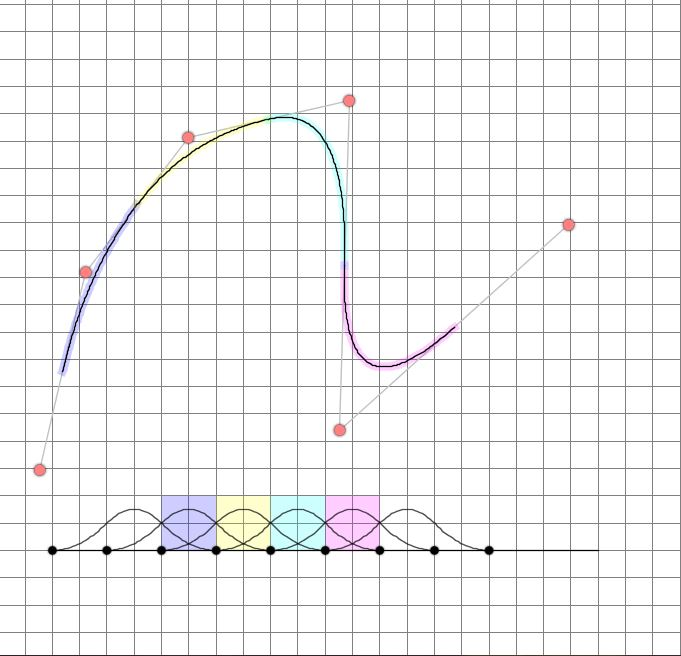
\includegraphics[width=0.45\textwidth]
{pics/Grundlagen/bspline_uniform}\label{fig:bspline_uniform}}
\quad
\subfloat[Endpunktinterpolation, Grad 2]{
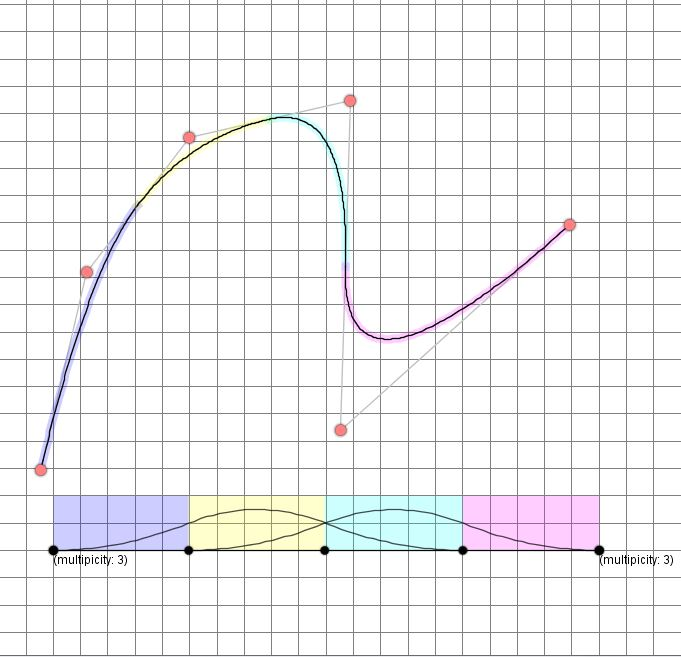
\includegraphics[width=0.45\textwidth]
{pics/Grundlagen/bspline_endpoint_interpolation}\label{fig:bspline_inter_2}}
\quad
\subfloat[Zuf�llig verteilter Knotenvektor]{
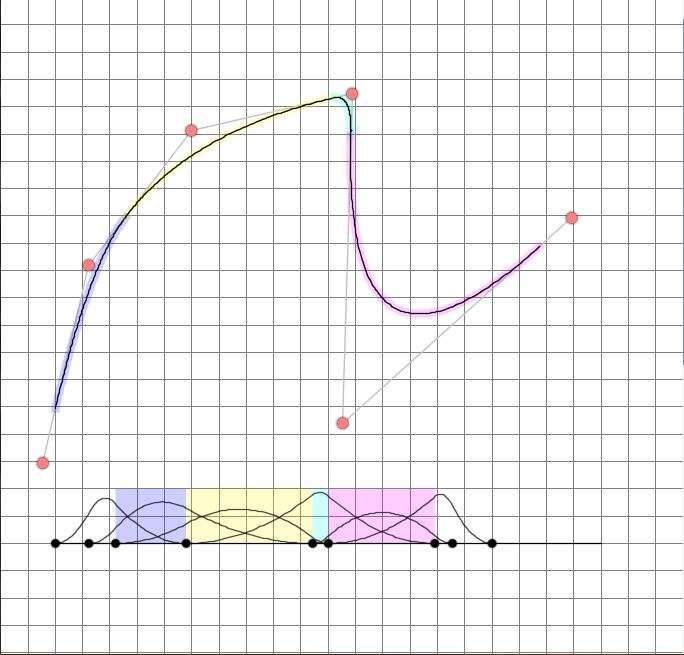
\includegraphics[width=0.45\textwidth]
{pics/Grundlagen/bspline_random}\label{fig:bspline_random}}
\quad
\subfloat[Endpunktinterpolation, Grad 4]{
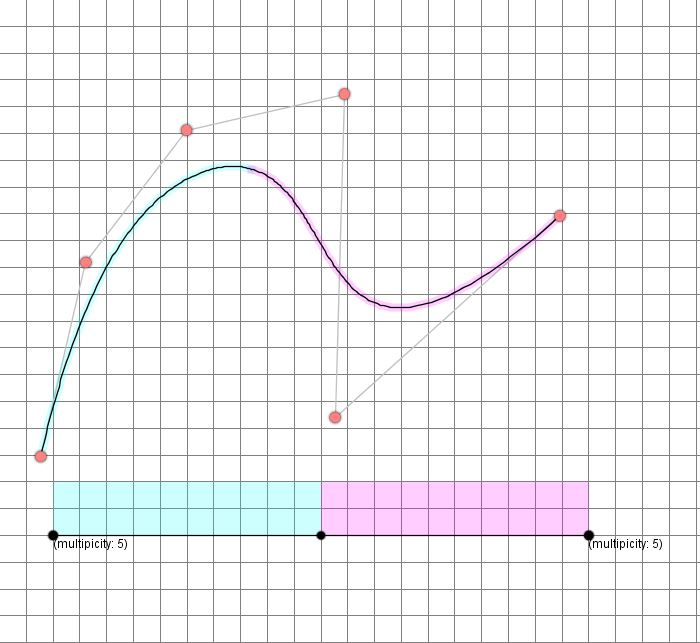
\includegraphics[width=0.45\textwidth]
{pics/Grundlagen/bspline_endpoint_deg4}\label{fig:bspline_inter_4}}
\quad
\caption[Beispiele Bsplines]{Unterschiedliche Bsplines, abh�ngig von Grad und Verteilung auf Knotenvektor. Die Farbe des Bspline Teilst�cks verweist auf das entsprechende Teilintervall auf dem Knotenvektor. \label{fig:bsplines_example}}
\end{figure}

\section{Color Deconvolution}\label{sec:color_deconvolution}

Die sogenannte Color Deconvolution ist eine Farbraumtransformation spezifisch f�r die Pathologie bzw. H�motologie, da hier Farbstoffe zum Einsatz kommen. Das Ziel ist es, das Bild durch eben diese F�rbemittel auszudr�cken. \citeeig{ruifrok2001quantification} schlagen dieses Verfahren vor, mit dem Ziel genauere Aussagen �ber die F�rbung machen zu k�nnen. Die maximale Anzahl verschiedener Farbstoffe ist dabei drei, da eine h�here Anzahl, den Transfer aus einem  trichromatischem Farbraum in einen h�herdimensionalen Raum bedeuten w�rde. 

Die Absorption von Licht durch das chemische Mittel folgt dem Lambert-Beerschen-Gesetz (\ref{equ:lambert_beer}), wobei $I_k$ als die Lichtintensit�t nach Passieren der Probe und $I_{0,k}$ vor der Probe festgelegt ist. Der Index $k$ steht f�r den detektierenden Kanal, also R,G oder B. $A$ entspricht der Menge an F�rbemittel und  $c_k$ dem Absorptionsfaktor. 

\begin{equation}\label{equ:lambert_beer}
I_k = I_{0,k}e^{-Ac_k}
\end{equation} 

Der Zusammenhang zwischen der Menge an Farbstoff und der detektierten Intensit�t ist also nicht linear. Aus diesem Grund wird das Bild zun�chst mit Hilfe des Logarithmus in den sogenannten OD-Raum (Optical Density) transferiert \ref{equ:od}.

\begin{equation}\label{equ:od}
OD_k = -log\left(\frac{I_k}{I_{0,k}}\right) = Ac_k
\end{equation} 


\citeeig{khan2014nonlinear} dr�cken die Zusammenh�nge f�r die Color Deconvolution in Anlehnung an \citeauthor{ruifrok2001quantification} in Matrixschreibweise folgenderma�en aus:

\begin{equation}\label{equ:beer_matrix}
\Psi = e^{-\mathbf{S}\hat\Psi} 
\end{equation}

In Gleichung \ref{equ:beer_matrix} steht $\mathbf{S}$ f�r die sogenannte Stainmatrix, welche in Formel \ref{equ:stainmatrix} genauer beschrieben wird. Sie beinhaltet die Absorptionsfaktoren der vorkommenden Farbstoffe f�r die einzelnen Kan�le. $\Psi$ beschreibt den urspr�nglichen Farbraum, also RGB und $\hat\Psi$ den neuen Farbraum. 

\begin{equation}\label{equ:stainmatrix}
\mathbf{S} =
\begin{bmatrix}
\bar s_{r,1} & \bar s_{g,1} & \bar s_{b,1}\\
\bar s_{r,2} & \bar s_{g,2} & \bar s_{b,2}\\
\bar s_{r,3} & \bar s_{g,3} & \bar s_{b,3}
\end{bmatrix}
\end{equation}

Formel \ref{equ:beer_matrix} l�sst sich umstellen nach $\hat\Psi$ \ref{equ:color_deconvolution}

\begin{align}\label{equ:color_deconvolution}
&\textrm{} &&\hat\Psi(c)= \mathbf{D}\Phi(c) \\
&\textrm{Es gelten } &&\mathbf{D}= \mathbf{S}^{-1} \\
&\textrm{und } &&\Phi(c) = - log(\Psi(c))
\end{align}

Der hier als $\Phi$ bezeichnete Farbraum beschreibt damit den OD-Wert (\ref{equ:od}). 
Ein entscheidender Punkt bei CD liegt in der Bestimmung der Stainvektoren. Im  Folgenden wird eine durch \citeauthor{ruifrok2001quantification} beschriebene M�glichkeit vorgestellt, wie diese manuell f�r eine spezifische F�rbung gefunden werden. Dabei sollen Proben mit nur einem der sp�ter verwendeten Farbstoffe untersucht werden. Im OD-Raum ergibt sich an den gef�rbten Stellen ein Farbvektor, bei dem die L�nge linear zur Menge an Farbstoff ist. Ein eindeutiger Farbvektor ergibt sich aus diesem Grund durch Normieren des Farbvektors im OD-Raum. \citeauthor{ruifrok2001quantification} f�hrten das Verfahren f�r eine F�rbung mit H�matoxylin, Eosin und DAB durch. Die Matrix vor und nach dem Normierungsschritt sind in Formel \ref{equ:stain_hedab} gezeigt. Die Stainvektoren der einzelnen Farbstoffe entsprechen dabei den Zeilen der Matrix.

\begin{align}\label{equ:stain_hedab}
\mathbf{S} & = 
\begin{bmatrix}
0.18 & 0.20 & 0.08\\
0.01 & 0.13 & 0.01\\
0.10 & 0.21 & 0.29
\end{bmatrix}
\\
\mathbf{S_{norm}} & = 
\begin{bmatrix}
0.65 & 0.70 & 0.29\\
0.07 & 0.99 & 0.11\\
0.27 & 0.57 & 0.78
\end{bmatrix}\nonumber
\end{align}

F�r eine bestimmte F�rbemethode sind die so ermittelten Werte eine N�herung, weil sich die Stainvekoren leicht �ndern k�nnen, je nach verwendeter Kamera, Lichtquelle und dem Alter der Proben. Die optimalen Stainvektoren sind von Bild zu Bild leicht unterschiedlich, auch wenn die gleichen Farbstoffe verwendet wurden. Ans�tze um exakte und bildspezifische Werte zu finden werden in den Abschnitten \ref{sec:macenko} und \ref{sec:khan} beschrieben.  


\chapter[Stand der Technik]{Stand der Technik}\label{sec:stand_der_technik}
Das grunds�tzliche Ziel beim Einsatz von Algorithmen zur Farbnormalisierung ist, dass Objekte gleicher Farbe auch �hnliche Pixelwerte haben. Dies sollte unabh�ngig von der Beleuchtung im Bild sein. Beim Anwendungsfeld der Mikroskopie kommen als Faktoren zus�tzlich noch Probendicke und Farbstoffmenge hinzu. Im folgenden Kapitel soll ein �berblick �ber bestehende Verfahren gegeben werden, wobei der Schwerpunkt, die Normalisierung auf mikroskopischen Bildern, in Abschnitt \ref{sec:mikroskopie_normalisierung} behandelt wird. Zun�chst soll jedoch auf Methoden eingegangen werden, welche zwar oft eingesetzt werden, im vorliegenden Fall aufgrund der speziellen Bildakquisition jedoch ungeeignet sind. 
%\section[Allgemeine Farbnormalisierung]{Allgemeine Farbnormalisierung}%\label{sec:allgemeine_normalisierung}
%\color{red}
%Gray World Assumption, Farbkonstanz

%Referenz auf MA Bindl?
%\color{black}

\section{Farbkonstanzalgorithmen}\label{sec:farbkonstanz}
Das menschliche Gehirn ist innerhalb gewisser Grenzen in der Lage, die Farbe eines Objektes unabh�ngig von dessen Beleuchtung zu bestimmen. Diese F�higkeit ist die Grundlage f�r eine Gruppe von Ans�tzen, die als Farbkonstanzalgorithmen bezeichnet werden.

Das menschliche Auge ist das Vorbild f�r den sogenannten LMS-Farbraum. Die drei Kan�le entsprechen dabei den unterschiedlichen Zapfen, die auf lang-, mittel- und kurzwelliges Licht reagieren. Nach den Erkenntnissen von Johannes von Kries werden die unterschiedlichen Signale unabh�ngig voneinander vom Gehirn angepasst. Dieser Zusammenhang wird in der folgenden Formel \ref{equ:kries} dargestellt.
\begin{align}\label{equ:kries}
L_{a} & = k_{L}L\\
M_{a} & = k_{M}M\\
S_{a} & = k_{S}S
\end{align}
$L_{a}$, $M_{a}$ und $S_{a}$ sind hierbei die angepassten Signale. $k_{L}$, $K_{M}$ und $k_{S}$ sind hingegen die unabh�ngigen Skalierungsfaktoren.
%F�r die Bestimmung dieser Faktoren gibt es unterschiedliche M�glichkeiten. Zum einen k�nnen sie die Inversen des angenommenen Wei�punktes der Szene sein, zum anderen als Inverse des jeweils maximalen Werts des Kanals.
Eine Annahme die gerne gemacht wird um diese Faktoren zu finden, ist die sogenannte "Grey World Assumption". Im Kern wird davon ausgegangen, dass die durchschnittliche Reflektanz in einer Szene Grau entspricht. \color{red} Achtung dies ist ein w�rtliches Zitat aus MA Bindl, abkl�ren inwieweit zitierf�hig \color{black} Variationen gibt es u.a. bei der Wahl von Grau. 
Im einfachsten Fall k�nnen die Skalierungsfaktoren entsprechend \label{equ:grey_world} berechnet werden. Hierbei entspricht $m_{L1}$ dem Mittelwert des L-Kanals einer Referenzaufnahme, $m_{L2}$ dem Mittelwert des L-Kanals aus einer Testaufnahme, usw.  
\begin{align}\label{equ:grey_world}
k_{L}L & = \frac{m_{L2}}{m_{L1}}\\
k_{M}M & = \frac{m_{M2}}{m_{M1}}\\
k_{S}S & = \frac{m_{S2}}{m_{S1}}
\end{align}

Farbkonstanzmodelle treffen Annahmen �ber das Verhalten von reflektiertem Licht, was sie ungeeignet f�r die Mikroskopie macht, da hier transmittiertes Licht detektiert wird \cite{khan2014nonlinear}

\section[Farbnormalisierung in der Mikroskopie]{Farbnormalisierung in der Mikroskopie}\label{sec:mikroskopie_normalisierung}
F�r Farbnormalisierung im vorliegenden Anwendungsgebiet wird in der Regel der Ansatz verfolgt, ein Bild an ein gegebenes Referenzbild anzugleichen. 
W�hrend die Methoden in den Abschnitten \ref{sec:farbranking} und \ref{sec:color_deconvolution} eine Farbraumtransformation erfordern, ben�tigt das Farbranking (\ref{sec:farbranking}) keine Vorverarbeitungsschritte.

\subsection{Farbranking}\label{sec:farbranking}
Farbranking ist ein Verfahren, das von \citeeig{kothari2011automatic} eingef�hrt wurde. Hierbei werden zun�chst die Intensit�ten in allen Kan�len jeweils f�r das Eingangs- und Ausgangsbild sortiert. Anschlie�end werden f�r jedes Pixel zun�chst die Positionen in den sortierten Listen ermittelt. Die Farbintensit�ten bekommen am Ende die Werte zugewiesen, welche sich in den Listen des Referenzbildes an den gleichen Stellen befinden. Dieser Zusammenhang ist in Graphik \ref{fig:farbranking} f�r den Fall von Grauwertbildern mit Gr��e 3x3 dargestellt. Dabei entspricht Bild A dem Referenzbild und Bild B dem Eingangsbild. B' beschreibt das angepasste Ausgabebild. 

\begin{figure}[h]
\center
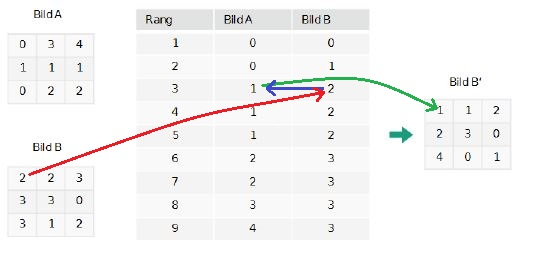
\includegraphics[width = 0.9\textwidth]{pics/StandTechnik/Farbranking_Ablauf}
\caption[Farbranking]{Links sind Eingangs- und Referenzbild dargestellt, in der Mitte die sortierten Listen und rechts das Ausgabebild. Die farbigen Pfeile sollen den Ablauf nach dem Erstellen der sortierten Listen verdeutlichen. Dabei wird der Pixel links oben im Bild behandelt. Rot: Finden des Pixelwertes in der sortierten Liste. Blau: Wahl des positionsgleichen Wertes aus dem Referenzbild. Gr�n: �bertrag dieses Wertes an die gleiche Stelle in Bild B' \label{fig:farbranking}}
\end{figure}

Die Schw�chen des Verfahrens, zeigen sich vor allem, wenn sich Eingangs- und Referenzbild zu sehr unterscheiden. In diesem Fall kommt es zu Artefakten, bei denen monochrome Fl�chen nach der Anpassung starke Unterschiede aufweisen.

\color{red}
evtl. Beispielbild
\color{black}

\subsection[Farbtransfer nach Reinhard]{Farbtransfer nach Reinhard}\label{sec:reinhard}
Ein andere Methode bei der die Akquisition keine Rolle spielt, wird von \citeeig{reinhard2001color} vorgeschlagen. Das Ziel ist es, die Anpassung in m�glichst schwach korrelierenden Kan�len durchzuf�hren. Ein Farbraum, der diese Eigenschaft f�r nat�rliche Bilder erf�llt ist der von \citeeig{ruderman1998statistics} vorgeschlagene $l\alpha\beta$-Raum. Die Umrechnung erfolgt dabei in mehreren Schritten. 
\begin{itemize}
\item{RGB $\rightarrow$ XYZ(Tristimulusraum): 
\begin{equation}\label{equ:rgb_xyz}
\begin{bmatrix}
X\\Y\\Z
\end{bmatrix}
= 
\begin{bmatrix}
0.5141 & 0.3239 & 0.1604\\
0.2651 & 0.6702 & 0.0641\\
0.0241 & 0.1228 & 0.8444
\end{bmatrix}
\begin{bmatrix}
R\\G\\B
\end{bmatrix}
\end{equation}
}
\item{XYZ $\rightarrow$ LMS\ref{sec:farbkonstanz}}

\begin{equation}\label{equ:xyz_lms}
\begin{bmatrix}
L\\M\\S
\end{bmatrix}
= 
\begin{bmatrix}
0.3897 & 0.6890 & -0.0787\\
-0.2298 & 1.1834 & 0.0464\\
0.000 & 0.000 & 1.0000
\end{bmatrix}
\begin{bmatrix}
X\\Y\\Z
\end{bmatrix}
\end{equation}
\item{Logarithmus auf dem LMS-Raum}
\item{Logarithmierter LMS $\rightarrow L\alpha\beta$}

\begin{equation}\label{equ:lms_lab}
\begin{bmatrix}
L\\\alpha\\\beta
\end{bmatrix}
= 
\begin{bmatrix}
\frac{1}{\sqrt{3}} & 0 & 0\\
0 & \frac{1}{\sqrt{6}} & 0\\
0 & 0 & \frac{1}{\sqrt{2}}
\end{bmatrix}
\begin{bmatrix}
1 & 1 & 1\\
1 & 1 & -2\\
1 & -1 & 0
\end{bmatrix}
\begin{bmatrix}
log(L)\\log(M)\\log(S)
\end{bmatrix}
\end{equation}
\end{itemize}

Die Umrechnung in \ref{equ:lms_lab} basiert auf einer Hauptachsentransformation, welche von \citeauthor{rudermann1998statistics} auf einem Datensatz nat�rlicher Fotos durchgef�hrt wurde. Die Eigenvektoren der gemittelten Kovarianzmatrix finden sich in der Rotationsmatrix dieser Transformation. \citeeig{reinhard2001color} schlagen vor, die Histogramme der dekorrelierten Kan�le mittels �bertragung von Mittelwert und Standardabweichung einzeln anzupassen\ref{sec:mean_std}.

\subsection{Color Deconvolution}\label{sec:color_deconvolution}
Die sogenannte Color Deconvolution ist spezifisch f�r die Pathologie bzw. H�motologie, da hier Farbstoffe zum Einsatz kommen. Das Ziel ist es, das Bild durch eben diese F�rbemittel auszudr�cken. \citeeig{ruifrok2001quantification} schlagen dieses Verfahren vor, mit dem Ziel quantitative Aussagen �ber die F�rbung machen zu k�nnen. Die maximale Anzahl verschiedener Farbstoffe ist dabei drei, da eine h�here Anzahl, den Transfer aus einem  trichromatischem Farbraum in einen h�herdimensionalen Raum bedeuten w�rde. 

Die Absorption von Licht durch das chemische Mittel folgt dem Lambert-Beerschen-Gesetz \ref{equ:lambert_beer}, wobei $I_k$ als die Lichtintensit�t nach Passieren der Probe und $I_{0,k}$ vor der Probe festgelegt ist. Der Index $k$ steht f�r den detektierenden Kanal, also R,G oder B. $A$ entspricht der Menge an F�rbemittel und  $c_k$ dem Absorptionsfaktor. 

\begin{equation}\label{equ:lambert_beer}
I_k = I_{0,k}e^{-Ac_k}
\end{equation} 

Der Zusammenhang zwischen der Menge an Farbstoff und der detektierten Intensit�t ist also nicht linear. Aus diesem Grund wird das Bild zun�chst mit Hilfe des Logarithmus in den sogenannten OD-Raum (Optical Density) transferiert \ref{equ:od}.

\begin{equation}\label{equ:od}
OD_k = -log\left(\frac{I_k}{I_{0,k}}\right) = Ac_k
\end{equation} 


\citeeig{khan2014nonlinear} dr�cken die Zusammenh�nge f�r die Color Deconvolution in Anlehnung an \citeauthor{ruifrok2001quantification} in Matrixschreibweise folgenderma�en aus:

\begin{equation}\label{equ:beer_matrix}
\Psi = e^{-\mathbf{S}\hat\Psi} 
\end{equation}

In Formel \ref{equ:beer_matrix} steht $\mathbf{S}$ f�r die sogenannte Stainmatrix, welche in Formel \ref{equ:stainmatrix} noch genauer beschrieben wird. Sie beinhaltet die Absorptionsfaktoren der vorkommenden Farbstoffe f�r die einzelnen Kan�le. $\Psi$ beschreibt den urspr�nglichen Farbraum, also RGB und $\hat\Psi$ den neuen Farbraum. 

\begin{equation}\label{equ:stainmatrix}
\mathbf{S} =
\begin{bmatrix}
\bar s_{r,1} & \bar s_{g,1} & \bar s_{b,1}\\
\bar s_{r,2} & \bar s_{g,2} & \bar s_{b,2}\\
\bar s_{r,3} & \bar s_{g,3} & \bar s_{b,3}
\end{bmatrix}
\end{equation}

Formel \ref{equ:beer_matrix} l�sst sich umstellen nach $\hat\Psi$ \ref{equ:color_deconvolution}

\begin{align}\label{equ:color_deconvolution}
&\textrm{} &&\hat\Psi(c)= \mathbf{D}\Phi(c) \\
&\textrm{Es gelten } &&\mathbf{D}= \mathbf{S}^{-1} \\
&\textrm{und } &&\Phi(c) = - log(\Psi(c))
\end{align}

Der hier als $\Phi$ bezeichnete Farbraum beschreibt damit den OD-Wert(\ref{equ:od}). 
Ein entscheidender Punkt bei CD liegt in der Bestimmung der Stainvektoren. In den folgenden Abschnitten \ref{sec:stains_f�rbung} und \ref{sec:stains_bild} werden unterschiedliche M�glichkeiten vorgestellt, diese zu bestimmen.

\subsubsection{Stainvektoren f�r eine F�rbung}\label{sec:stains_f�rbung}
Ein Ansatz an die Stainvektoren f�r eine F�rbemethode und einen Versuchsaufbau zu kommen, wird von \citeauthor{ruifrok2001quantification} vorgeschlagen. Dabei sollen Proben mit nur einem der sp�ter verwendeten Farbstoffe untersucht werden. Im OD-Raum ergibt sich an den gef�rbten Stellen ein Farbvektor, bei dem die L�nge linear zur Menge an Farbstoff ist. Ein eindeutiger Farbvektor ergibt sich aus diesem Grund durch Normieren des Farbvektors im OD-Raum. \citeauthor{ruifrok2001quantification} f�hrten das Verfahren f�r eine F�rbung mit H�matoxylin, Eosin und DAB durch. Die Matrix vor und nach dem Normierungsschritt sind in Formel \ref{equ:stain_hedab} gezeigt. Die Stainvektoren der einzelnen Farbstoffe entsprechen dabei den Zeilen der Matrix.

\begin{align}\label{equ:stain_hedab}
\mathbf{S} & = 
\begin{bmatrix}
0.18 & 0.20 & 0.08\\
0.01 & 0.13 & 0.01\\
0.10 & 0.21 & 0.29
\end{bmatrix}
\\
\mathbf{S_{norm}} & = 
\begin{bmatrix}
0.65 & 0.70 & 0.29\\
0.07 & 0.99 & 0.11\\
0.27 & 0.57 & 0.78
\end{bmatrix}\nonumber
\end{align}

F�r eine bestimmte F�rbemethode sind die so ermittelten Werte eine N�herung, wobei sich die Stainvekoren leicht �ndern k�nnen, je nach verwendeter Kamera, Lichtquelle und dem Alter der Proben. Die optimalen Stainvektoren sind also von Bild zu Bild leicht unterschiedlich, auch wenn die gleichen Farbstoffe verwendet wurden.  

\subsubsection{Spezifische Stainvektoren f�r ein Bild}\label{sec:stains_bild}

Es gibt Versuche, die Vektoren f�r jedes Bild neu zu bestimmen, welche implizit davon ausgehen, dass es Pixel im Bild gibt, welche eindeutig einem Farbstoff zuzuordnen sind. Es sollte also Stellen geben, an denen keine �berlappung stattfindet. 

\paragraph{Macenko}\label{sec:macenko}

Zun�chst einmal soll der Vorschlag von \citeeig{macenko2009method} vorgestellt werden, welcher die folgenden Schritte umfasst:
\begin{itemize}
\item{Start: RGB-Bild}
\item{RGB $\rightarrow$ OD}
\item{Betrachten aller Werte mit OD-Intensit�t gr��er einem Schwellwert $\beta$, wobei 0.15 empirisch als optimaler Schwellwert bestimmt wurde. Durch dieses Vorgehen sollen nur Pixel mit relevanter Farbinformation ber�cksichtigt werden.}
\item{Berechnen der Korrelationsmatrix und der zugeh�rigen SVD(Singular Value Decomposition)}
\item{Berechnen einer Ebene aus den zwei Eigenvektoren, die zu den beiden gr��ten Eigenwerten geh�ren.}
\item{Projektion aller OD-Pixel auf diese Ebene}
\item{Histogramm �ber die Winkel, welche die projizierten Pixel mit dem ersten Eigenvektor einschlie�en}
\item{Bestimmen des robusten Minimum und Maximum in diesem Histogramm}
\item{R�cktransformation in den OD-Raum, Minimum und Maximum entsprechen den Stainvektoren}
\end{itemize} 

Die Logik hinter diesem Vorgehen ist, dass durch das W�hlen von Minimum und Maximum, jeder Wert dazwischen als lineare Summe dieser beiden Vektoren ausdr�ckbar ist. Abbildung \ref{fig:hist_angle} zeigt ein Beispiel f�r ein Histogramm �ber die Winkel, Grafik \ref{fig:hist_angle} zeigt das Ergebnis einer Color Deconvolution mit den gefundenen Stainvektoren.
\begin{figure}[h]
\center
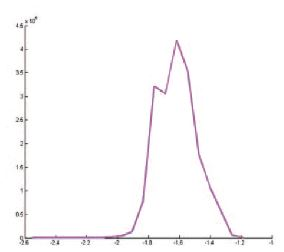
\includegraphics[width = 0.5\textwidth]
{pics/StandTechnik/hist_angle_macenko}
\caption[Winkelhistogramm Macenko]{Beispiel f�r ein Histogramm �ber die Winkel, welche die projizierten Punkte mit der ersten Hauptachse einschlie�en. Daraus zu bestimmen sind das robuste Minimum und Maximum.\label{fig:hist_angle} }
\end{figure}
\begin{figure}[h]
\center
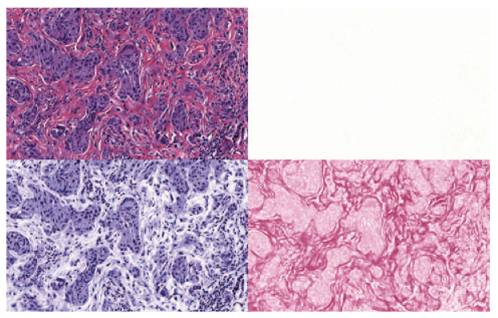
\includegraphics[width = 0.9\textwidth]
{pics/StandTechnik/cd_macenko}
\caption[Color Deconvolution nach Macenko]{Links oben: originales Bild, unten das Bild aufgeteilt nach den beiden Grundfarbstoffen. Dritter Kanal rechts oben, welcher in diesem Beispiel fast leer erscheint.\label{fig:cd_macenko} }
\end{figure}

\citeauthor{macenko2009method} liefern auch einen Ansatz f�r die Normalisierung. Hierbei wird f�r jeden vorkommenden Farbstoff ein Histogramm berechnet, welches jedoch nur jene Pixel ber�cksichtigt, die �berwiegend diesen Farbstoff beinhalten.
Die Histogramme werden anschlie�end so skaliert, dass alle das gleiche Pseudomaximum haben um sie miteinander vergleichbar zu machen\ref{sec:skalierung}. Hierbei wird vor allem ber�cksichtigt, dass Proben gebleicht worden sein k�nnten und dieser Effekt reduziert. Allerdings wird nicht ber�cksichtigt, dass sich die Proben auch inhaltlich stark unterscheiden k�nnten. Das Ergebnis der Anpassung zweier Bilder ist in Grafik \ref{fig:macenko_result} gezeigt.

\begin{figure}[h]\centering
\subfloat[Originale Bilder]{
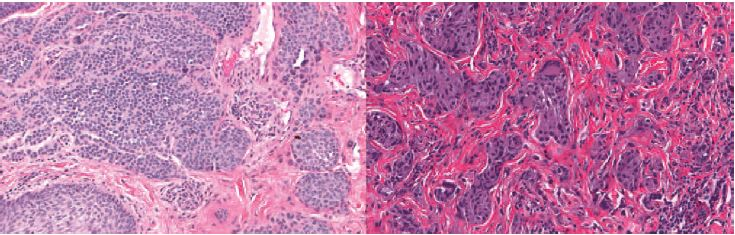
\includegraphics[width=0.9\textwidth]
{pics/StandTechnik/macenko_src}\label{fig:macenko_src}}
\quad
\subfloat[Farbnormalisierte Bilder]{
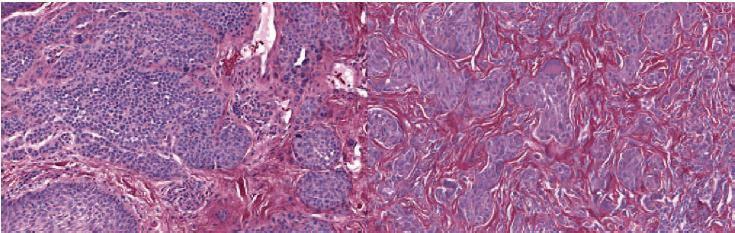
\includegraphics[width=0.9\textwidth]
{pics/StandTechnik/macenko_norm}\label{fig:macenko_norm}}
\quad
\caption[Beispiel Farbnormalisierung Macenko]{In der oberen Zeile sind zwei verschiedene, originale h�matologische Bilder zu sehen, welche beide mit H�matoxylin und Eosin gef�rbt wurden, aber trotzdem deutliche Unterschiede in der Erscheinung aufweisen. Unten ist das Ergebnis der Normalisierung zu sehen. \label{fig:macenko_result}}
\end{figure}

\paragraph{Khan}\label{sec:khan}

Eine andere Methode, welche auf Maschinellem Lernen basiert, wird von \citeeig{khan2014nonlinear} vorgeschlagen. Hierbei soll ein Klassifikator trainiert werden, welcher f�r jedes Pixel angibt, von welchem Farbstoff es mehrheitlich gepr�gt ist, bzw. ob es zum Hintergrund geh�rt.

\citeauthor{khan2014nonlinear} f�hren als bildspezifisches Merkmal einen sogenannten "Stain Color Descriptor"(SCD) ein.
Sei

$\mathbf{I} = \lbrace I_1,I_2,\ldots,I_k \rbrace$,

ein Set von $k$ Trainingsbildern, dann gibt es ein Set korrespondierender SCDs

$\mathbf{\hat H} = \lbrace \hat{H_1},\hat{H_1},\ldots,\hat{H_k}\rbrace$.

Hierf�r werden zun�chst alle Trainingsbilder mit Hilfe eines Octree quantisiert (Abbildung \ref{fig:octree}). Der Farbraum wird zun�chst in acht Unterr�ume unterteilt, was durch eine gleichm��ige Unterteilung jedes Farbkanals in zwei Bereiche erreicht wird. Diese Unterr�ume werden rekursiv wieder in acht Teile zerlegt, bis die Anzahl an Pixeln, die durch diesen Bereich repr�sentiert werden unterhalb eines Grenzwert liegt. 
\begin{figure}
\center
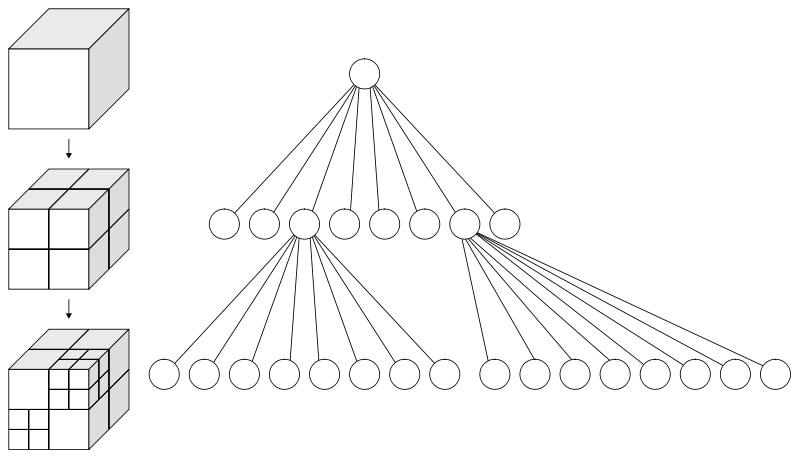
\includegraphics[width = 0.6\textwidth]
{pics/StandTechnik/octree}
\caption[Schema Octree]{Aufbau eines Octree: Baumstruktur, bei dem jeder Knoten, der kein Blatt ist, in acht Kindknoten zerlegt wird\cite{octree}. }\label{fig:octree}
\end{figure}
Das Ziel von \citeauthor{khan2014nonlinear} ist ein Baum mit 255 Bl�ttern \color{red}(rechnerisch gar nicht m�glich, $Sum != 1+x*7, x \in \mathbb{N}$)\color{black} weshalb nach der Zerlegung diejenigen Knoten mit der geringsten Zahl an Pixeln wieder zusammenf�gt werden, solange bis die gew�nschte Zahl erreicht ist.

Die Quantisierung jedes Bildes ergibt ein Set 
$\mathbf{H} = \lbrace H_1, H_2,\ldots,H_k$, wobei jedes Histogramm $H_i$ 255 Elemente hat. Zur Berechnung des korrespondierenden SCD $\hat{H_i}$ wird zun�chst ein mittlerer Vektor $\bar H$ und die Kovarianzmatrix $\Sigma_h$ berechnet. Um eine lineare Dimensionsreduktion durchzuf�hren wird die Eigenvektormatrix $\mathbf {E}^r_h$ bestimmt, wobei $r$ die Zieldimension darstellt. Die Autoren stellten dabei f�r $r \> 1$ keine signifikante Verbesserung der Klassifikationsergebnisse fest. Formel \ref{equ:khan_dimreduc} zeigt die Projektion eines Histograms $H_i$ in den $r$-dimensionalen Raum, welcher von den Eigenvektoren aufgespannt wird, die zu den $r$ gr��ten Eigenwerten geh�ren.
\begin{equation}\label{equ:khan_dimreduc}
\hat{H_i} = \mathbf{E}^r_h\left(H_i - \bar{H}\right)
\end{equation}

Der zur Zuordnung zu einer Klasse verwendete Merkmalsvektor ist folgenderma�en aufgebaut: $\mathcal{F} = \lbrack R,G,B, \hat{H} \rbrack$. Die Werte $R$,$G$ und $B$ entsprechen dabei den Werten aus den entsprechenden Kan�len eines RGB-Bildes. 
Die Wahrscheinlichkeit, mit der ein Pixel einem Farbstoff $s_n$ zuzuordnen ist, wird mittels Formel \ref{equ:khan_prob_output}
\begin{equation}\label{equ:khan_prob_output}
P(s_n \mid \mathcal{F}) = \frac{P_{s_n}(s_n\mid \mathcal{F})}{P_{s_1}(s_1\mid \mathcal{F})+P_{s_2}(s_2\mid \mathcal{F})+P_{s_{bgd}}(bgd\mid \mathcal{F})}
\end{equation}
Die berechnete Wahrscheinlichkeit wird f�r zwei verschiedene Zwecke genutzt:
\begin{itemize}
\item{Berechnung der normalisierten Stainvektoren f�r jede Klasse $s_n$.}
\item{Zuordnung zu einer Klasse $\theta(c) in \lbrace \text{GEF�RBT, HINTERGRUND, ANDERES}\rbrace$ mit Hilfe der folgenden Regel \ref{equ:thres_rule}:
\begin{align}\label{equ:thres_rule}
&if \quad P(bgd\mid\mathcal{F} > T_{bgd}:\quad &&\zeta(c)= \text{HINTERGRUND}\nonumber \\
&elseif \quad P(s_n\mid\mathcal{F} > T_{fgd}:\quad &&\zeta(c)= \text{STAINED}\\
&else \quad \quad &&\zeta(c) = \text{OTHER}\nonumber
\end{align}}
$T_{bgd}$ und $T_{fgd}$ sind dabei Grenzwerte f�r die jeweiligen Entscheidungen. \citeauthor{khan2014nonlinear} geben beide mit $0.75$ an und stellen fest, dass die Wahrscheinlichkeiten in den meisten F�llen entweder nahe $0$ bzw. $1$ liegen, weshalb die Grenzwerte sehr stabil sind.
\end{itemize} 

Eine �bersicht �ber den Klassifikationsvorgangs von \citeauthor{khan2014nonlinear} gibt Abbildung \ref{fig:khan_classifier}.
\begin{figure}[h]
\center
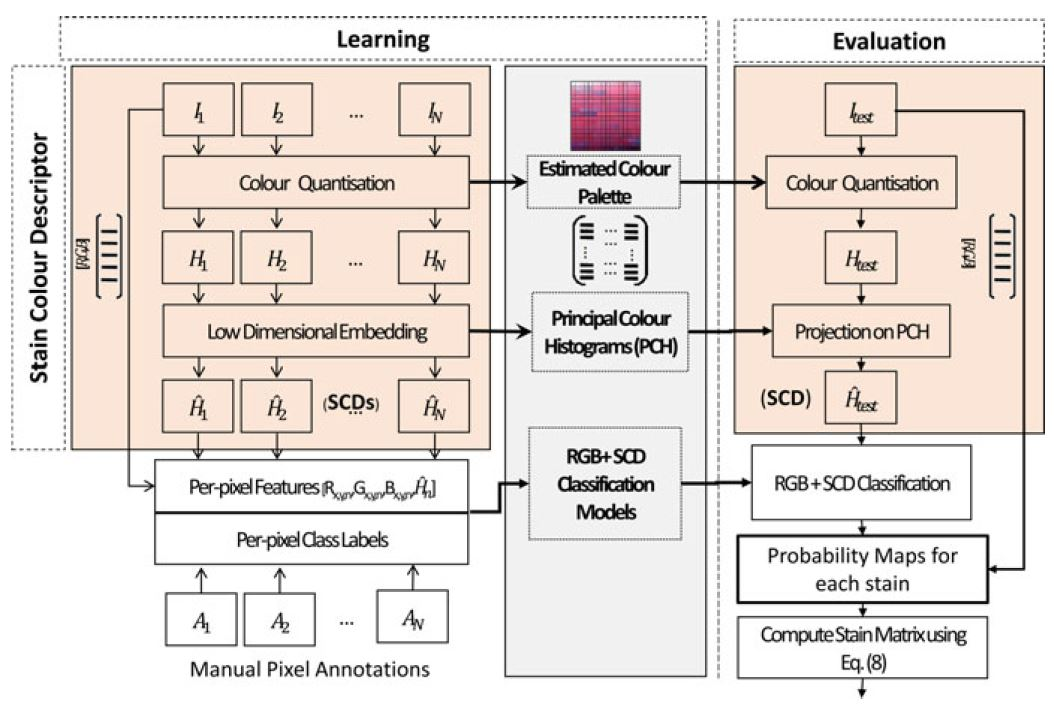
\includegraphics[width = 0.9\textwidth]
{pics/StandTechnik/khan_classifier}
\caption[Klassifikationsvorgang Khan]{�bersicht �ber den Klassifikationsansatz von \citeauthor{khan2014nonlinear}.\label{fig:khan_classifier} }
\end{figure}


\subsection{Histogrammanpassung}\label{sec:histogramm}
Histogramme sind eine M�glichkeit zur Beschreibung eines Bildes, weswegen viele Farbanpassungsalgorithmen darauf basieren, diese zu vereinheitlichen. Im folgenden sollen einige M�glichkeiten vorgestellt, wie diese Anpassung aussehen kann. Der Fokus liegt hierbei nicht auf einem verwendeten Farbraum, sondern darauf, wie die Histogramme beeinflusst werden. 

\subsubsection{Histogrammequalisierung}\label{sec:equalisierung}

Bei dieser Methode, wird eine Gleichverteilung f�r alle Intensit�ten angestrebt. Der Effekt wird sichtbar, wenn man das kumulative Histogramm betrachtet. Der Kurvenverlauf n�hert sich nach der Anpassung einer Ursprungsgerade an. Ein Beispiel wie sich die Anpassung auswirkt ist in Abbildung \ref{fig:EQGraubild} gezeigt.

\begin{figure}[h]\centering
\subfloat[Originales Grauwertbild\cite{url_unequ_image}]{
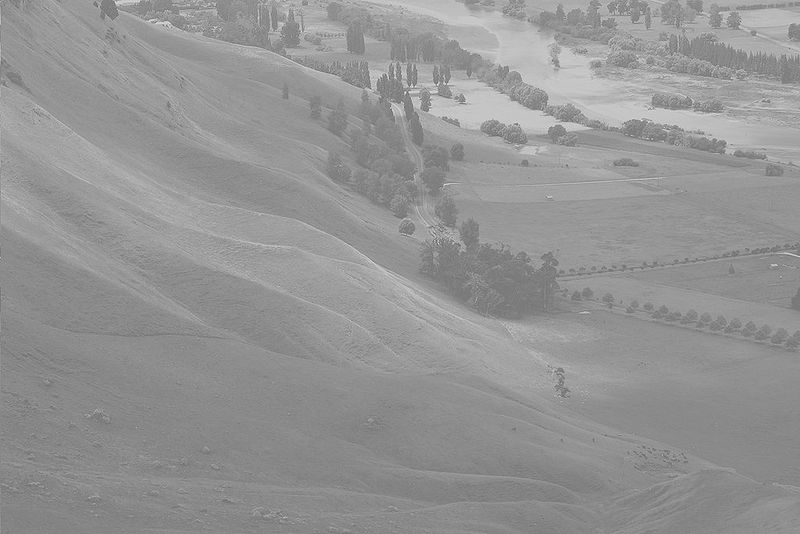
\includegraphics[width=0.45\textwidth]
{pics/StandTechnik/800px-Unequalized_Hawkes_Bay_NZ}\label{fig:unequalized}}
\quad
\subfloat[Originales Histogramm in roter Farbe und kumulatives Histogramm mit schwarzer Linie \cite{url_unequ_hist}.]{
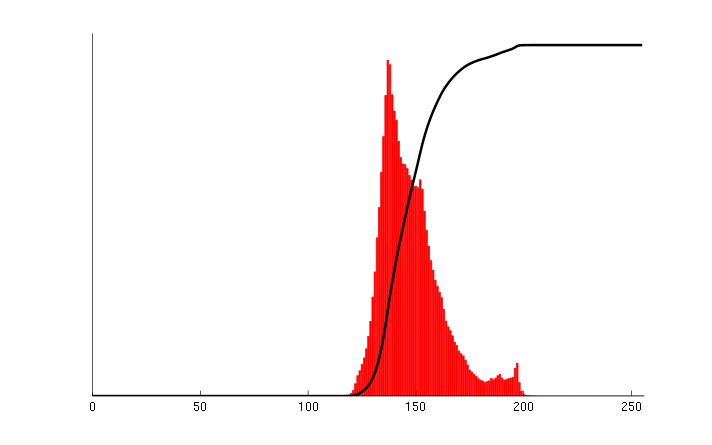
\includegraphics[width=0.45\textwidth]
{pics/StandTechnik/712px-Unequalized_Histogram}\label{fig:histoUn}}
\quad
\subfloat[Ausgeglichenes Grauwertbild \cite{url_equ_image}]{
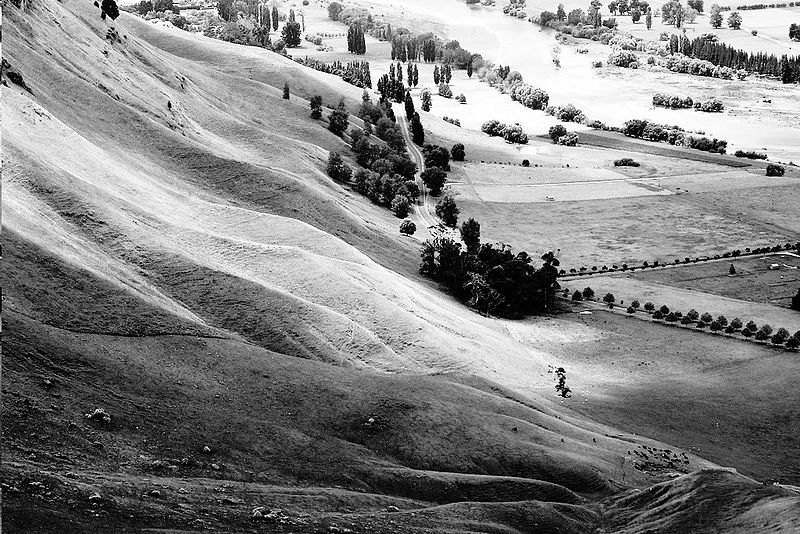
\includegraphics[width=0.45\textwidth]
{pics/StandTechnik/800px-Equalized_Hawkes_Bay_NZ}\label{fig:equalized}}
\quad
\subfloat[Ausgeglichenes Histogramm in Rot mit dem ann�hernd linearen kumulativen Histogramm in Schwarz \cite{url_equ_hist}]{
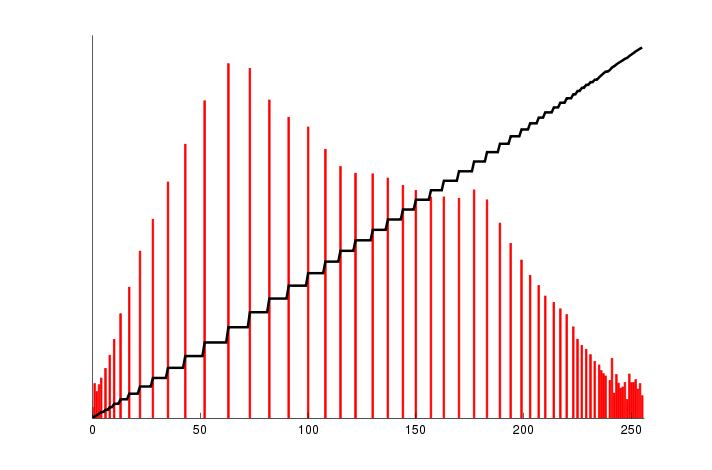
\includegraphics[width=0.45\textwidth]
{pics/StandTechnik/712px-Equalized_Histogram}\label{fig:histoEq}}
\quad
\caption[Beispiel einer Histogrammequalisierung]{Beispiel einer Histogrammequalisierung \label{fig:EQGraubild}}
\end{figure}


Im Gegensatz zu einem klassischem Histogramm, bei welchem die Anzahl bzw. der Anteil der Pixel mit einen bestimmten Wert betrachtet wird, werden hier die Pixel ber�cksichtigt, welche kleiner oder gleich diesem Wert sind. Der Verlauf eines kumulativen Histogramms ist aus diesem Grund immer monoton steigend.

\subsubsection{Histogrammspezifikation}\label{sec:spezifikation}

Auch bei der Histogrammspezifikation spielt das kumulative Histogramm eine wichtige Rolle. Im Gegensatz zur in Abschnitt \ref{sec:equalisierung} beschriebenen Equalisierung, ist der Zielverlauf der Kurve bei der Spezifikation keine Gerade, sondern das kumulative Histogramm eines Referenzbildes. Das Vorgehen soll durch die Abbildung \ref{fig:equalisierung} verdeutlicht werden. Zun�chst wird f�r einen Bin der Quelle der Dichtewert auf der y-Achse des Histogramms gesucht. Derjenige Intensit�tswert der Referenz, bei dem die Zielfunktion die gleiche Dichte aufweist, ist der gesuchte Transferwert.  
\begin{figure}[h]
\center
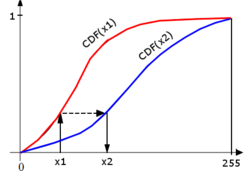
\includegraphics[width = 0.45\textwidth]
{pics/StandTechnik/250px-Histogram_matching}
\caption[Beispiel Histogramspezifikation]{Vorgang bei der Histogrammspezifikation. Die CDF(Cumulated Density Function) eines Bildes $\mathbf{x1}$ soll auf die CDF von Bild $\mathbf{x2}$ abgebildet werden. Die Pfeile verbildlichen dabei das genaue Vorgehen\cite{url_hist_spec}.\label{fig:equalisierung}}
\end{figure}

\subsubsection{Histogrammskalierung}\label{sec:skalierung}
Mit Hilfe von Skalierung kann ein beliebiges Maximum, welches ein Histogramm aufweisen soll, erzwungen werden. Als Zielmaximum kann der maximal m�gliche Wert angenommen werden (z.b. bei 8 Bit Farbtiefe 255), das Maximum eines Referenzhistogramms, der Durchschnitt der Maxima eines gr��eren Datensatzes oder ein willk�rlich festgelegter Wert. Angewendet wird das Verfahren u.a. von \citeauthor{macenko2009method}, wobei die vorausgehende Farbraumtransformation in Abschnitt \ref{sec:macenko} n�her beschrieben wird. Formel \ref{equ:scale} beschreibt den Zusammenhang zwischen einem angepassten Wert $\hat x_i$ und $x_i$. Der Skalierungsfaktor $k$ ergibt sich dabei aus dem Verh�ltnis zwischen $m_{ref}$, dem Zielmaximum, und $m$, das dem urspr�nglichem Maximum des zu ver�ndernden Histogramms entspricht. Gilt $k > 1$ wird das Histogramm gestreckt, bei $k < 1$ wird das Bild dagegen gestaucht.
\begin{equation}\label{equ:scale}
\hat x_i = \frac{m_{ref}}{m}x_i = kx_i
\end{equation}

\subsubsection{Anpassung von Mittelwert und Standardabweichung}\label{sec:mean_std}
Im vorherigen Abschnitt \ref{sec:skalierung} wurde das Maximum eines Histogramms angepasst. \citeeig{reinhard2001color} schlagen dagegen vor Mittelwert und Standardabweichung des Histogramms zu kontrollieren. W�hrend dies beim Mittelwert �ber eine einfache Verschiebung des Histogramms m�glich ist, wird f�r die Standardabweichung eine Stauchung bzw. Dehnung ben�tigt. Formel \ref{equ:mean_std} zeigt den allgemeinen Fall, wobei das Histogramm des Kanals $x$ einer Quelle $src$ dem �quivalenten Kanal der Referenz $ref$ nachempfunden werden soll. Das neue Histogramm wird als $neu$ bezeichnet. Au�erdem gilt, dass $\sigma_x$ der Standardabweichung entspricht und $\bar{x}$ dem Mittelwert.
\begin{align}\label{equ:mean_std}
x^{\star} &= x_{src} - \bar{x}_{src}\nonumber\\
\hat{x} &= \frac{\sigma_{x_{src}}}{\sigma_{x_{ref}}}\nonumber\\
x_{neu} &= \hat{x} + \bar{x}_{ref}
\end{align}
Ein Beispiel f�r die Anpassung nach Reinhard mit nat�rlichen Aufnahmen ist in Graphik \ref{fig:reinhard} zu sehen. 
\begin{figure}[h]
\center
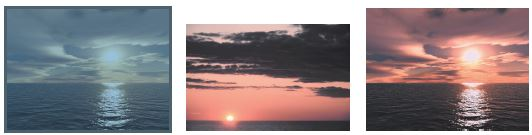
\includegraphics[width = 0.9\textwidth]
{pics/StandTechnik/Beispiel_reinhard}
\caption[Beispiel f�r Farbanpassung nach Reinhard]{Beispiel f�r die Farbanpassung nach Reinhard. Links sieht man das Eingabebild, in der Mitte die normalisierte Version und rechts das Referenzbild.\label{fig:reinhard} }
\end{figure}


\subsubsection{Bspline}\label{sec:bspline}
\citeeig{khan2014nonlinear} schlagen f�r die Anpassung der Histogramme Bsplines vor. Dieses Konzept erlaubt es Kurven zu modellieren, die ein Set von Kontrollpunkten mittels Teilpolynomen so ann�hert, dass sie an den Grenzen stetig sind. Der Grad der Stetigkeit ist dabei �ber den Grad des Bsplines $n$ festgesetzt. Die Kurve ist neben den Kontrollpunkten auch noch vom Knotenvektor $\mathbf{T} =  (t_i)$ beeinflusst, welcher die Parameterintervalle festlegt. Ein Beispiel eines Knotenvektors ist in Abbildung \ref{fig:knotvector} dargestellt.
\begin{figure}[h]
\center
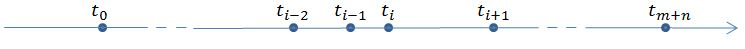
\includegraphics[width = 0.7\textwidth]
{pics/StandTechnik/knotvector}
\caption[Bspline Knotenvektor]{Grunds�tzlicher Aufbau eines Knotenvektors der L�nge $m+n+1$. $n$ ist der Grad des Bsplines und $m$ die Anzahl der Kontrollpunkte.\label{fig:knotvector}}
\end{figure}

Grundlage f�r einen Bspline sind die Basisfunktionen $n_i^k(u)$, die nach Formel \ref{equ:bspline_basis} definiert sind. 
\begin{align}\label{equ:bspline_basis}
N^0_i(u) & := 
\begin{cases}
1 &t_i \leq u \le t_{i+1}\\
0 &sonst
\end{cases}\\
N_i^k(u) & := \frac{u-t_i}{t_{i+k}}N^{k-1}_i(u)+\frac{t_{i+k+1}-u}{t_{i+k+1}-t_{i+1}}N^{k-1}_{i+1}(u), k =1,\ldots, n
\end{align}

Die Berechnung eines Bsplines $F$ mit Grad $n$, Kontrollpunkten $\mathbf{D} = \lbrace \mathbf{d}_0, \ldots \mathbf{d}_{m-1}$ und einem Knotenvektor $\mathbf{T}$ erfolgt nach Formel \ref{equ:bspline}
\begin{equation}\label{equ:bspline}
F(u) := \sum^{m-1}_{i=0} N^n_i(u)\mathbf{d}_i 
\end{equation}

Einige wichtige Eigenschaften eines Bsplines sind in der folgenden, nicht vollst�ndigen, Liste aufgef�hrt:
\begin{itemize}
\item{Keine Endpunktinterpolation}
\item{Fallen $n$ Knoten $t_i$ auf den gleichen Wert, so wird der zugeh�rige Kontrollpunkt interpoliert}
\item{Fallen $n$ Kontrollpunkte $\mathbf{d}_i$ auf den gleichen Punkt, so wird dieser interpoliert}
\item{Lokale Kontrolle: F�r $u \in \lbrack )$ ist die Kurve unabh�ngig von $\mathbf{d}_j$, wobei $j < i-n$ und $j > i$ gilt.}
\end{itemize}

Die Einsatzm�glichkeit dieses Konzeptes f�r eine Farbanpassung, liegt nun in der Definition der Kontrollpunkte durch Merkmale des Histogramms. Dabei setzt sich eine solche St�tzstelle aus einem Merkmal der Quelle, z.b. dem Mittelwert oder dem Maximum, und dem �quivalenten Merkmal der Referenz zusammen. \citeauthor{khan2014nonlinear} segmentieren das Bild zun�chst in drei Bereiche: Gef�rbt, Hintergrund und Anderes. Dabei nutzen sie die Ausgabe des Klassifikators, welcher in Abschnitt \ref{sec:khan} beschrieben wurde. Nachdem die Color Deconvolution durchgef�hrt wurde \ref{sec:color_deconvolution}, werden f�r jeden Kanal separat die Anpassung mittels Bspline festgelegt. Hierzu wird f�r jeden der drei segmentierten Bereiche ein Histogramm gebildet und das robuste Minimum und Maximum sowie der Mittelwert bestimmt (Abbildung \ref{fig:cd_histograms}). F�r jeden Kanal gibt es demnach neun Merkmale, was wiederum zu neun Kontrollpunkten f�r den Bspline f�hrt. Optisch bzw. chemisch ges�ttigte Pixel sollen nicht ver�ndert werden, weshalb zus�tzliche St�tzstellen entlang der Hauptachse eingef�hrt werden, damit die S�ttigungsstellen interpoliert werden. Der beispielhafte Verlauf eines Bsplines f�r einen Kanal ist in Abbildung \ref{fig:cd_bspline} gezeigt.
\begin{figure}[h]
\center
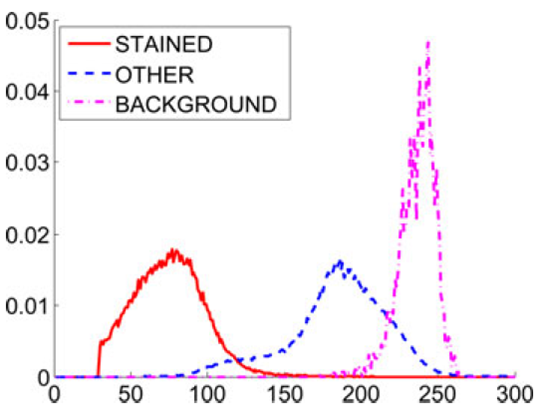
\includegraphics[width = 0.4\textwidth]
{pics/StandTechnik/cd_histograms}
\caption[Khan Histogramme]{Histogramme von drei verschiedene Regionen f�r einen Kanal nach CD.\label{fig:cd_histograms}}
\end{figure}
\begin{figure}[h]
\center
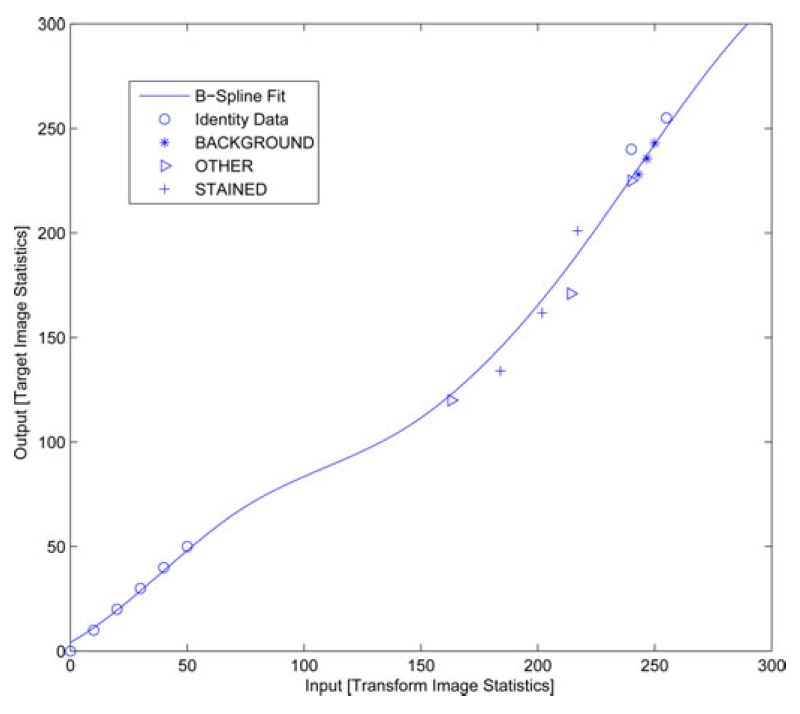
\includegraphics[width = 0.7\textwidth]
{pics/StandTechnik/cd_bspline}
\caption[Khan Bspline]{Bspline (blaue Linie) zur Anpassung eines CD-Kanals nach Khan. Auf der x-Achse der urspr�ngliche Wert des Quellbildes, auf der y-Achse der neue Wert. Die Kontrollpunkte aus den Histogrammmerkmalen, sowie die zus�tzlichen St�tzstellen, zur Sicherstellung der Interpolation der S�ttigungsstellen sind eingezeichnet.\label{fig:cd_bspline}}
\end{figure}

Eine Gesamt�bersicht �ber den Farbnormalisierungsansatz von Khan gibt Abbildung \ref{fig:khan_normalisation}. Dabei ist auch ein Beispiel f�r die Wirkung der Methode zu sehen.
\begin{figure}[h]
\center
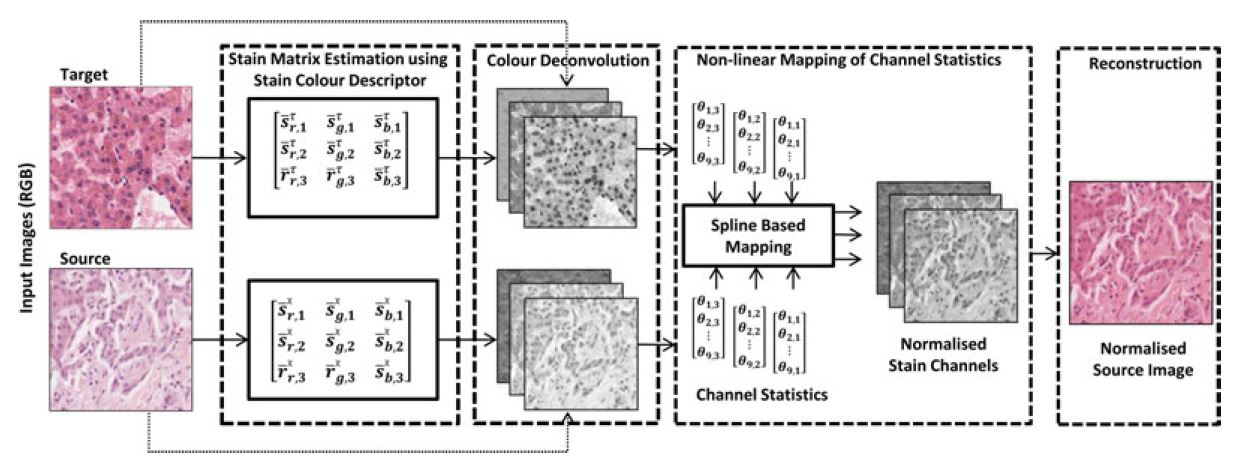
\includegraphics[width = 0.9\textwidth]
{pics/StandTechnik/khan_pipeline}
\caption[�bersicht Normalisierungsansatz Khan]{�bersicht �ber den Normalisierungsansatz von \citeauthor{khan2014nonlinear}.\label{fig:khan_normalisation} }
\end{figure}





\chapter[Material]{Material}\label{sec:material}
\chapter[Methoden]{Methoden}\label{sec:methoden}

\section{Implementierung Khan und Macenko}\label{sec:implementierung_khan_macenko}

\section{Eigener Workflow}\label{sec:eigener_workflow}

Im den folgenden Abschnitten soll aufgezeigt werden, inwiefern das Vorgehen von \citeauthor{khan2014nonlinear} und \citeauthor{macenko2009method} abge�ndert wurde um die aufgetretenen Probleme zu umgehen.

\subsection[Eigene Color Deconvolution]{Eigene Color Deconvolution}\label{sec:own_cd}
In n�chster N�herung wurden Stainvektoren f�r die F�rbung nach Giemsa (Methylenblau und Eosin) verwendet, welche von \citeeig{landini2016} nach dem in Abschnitt \ref{sec:stains_f�rbung} vorgestellten experimentellen Verfahren ermittelt wurden. F�r den fehlenden dritten Vektor, wird u.a. in der Arbeit von Khan angemerkt, dass dieser optimalerweise orthogonal zu den anderen beiden sein soll. Au�er im Fall von Einheitsvektoren, w�rde dieser jedoch negative Komponenten enthalten, was im Modell die Folge h�tte, dass die Absorption teilweise negativ w�re. Als L�sung wurden zwei verschiedene Ans�tze getestet. Die ersten beiden Zeilen der Stainmatrix sind bekannt und \citeauthor{landini2016} berechnet die dritte Zeile der Stainmatrix, in dem er zun�chst die Spalten normalisiert, f�r den Fall dass die ersten beiden Komponenten nicht schon �ber $1.0$ liegen. Tritt dies doch ein, so wird das Element der dritten Zeile auf $0.0$ gesetzt. Im n�chsten Schritt wird die Zeile normalisiert und Elemente die gleich $0$ werden zur Fehlerreduktion auf einen Wert $\epsilon = 0.01$ gesetzt. Diese Methode wurde der eigenen Idee gegen�bergestellt, bei der zun�chst �ber das Kreuzprodukt ein echt orthogonaler Vektor bestimmt wird. Dabei werden beide  Szenarien abh�ngig vom Vorzeichen ber�cksichtigt. Negative Komponenten werden auf $0.0$ gesetzt. Derjenige Vektor der nach dieser Operation die gr��ere L�nge aufweist, wird gew�hlt und normalisiert und als dritter Stainvektor eingesetzt. Unabh�ngig von der Wahl des dritten Vektors ist die Approximation f�r die vorhandenen Daten legitim, da der dritte Kanal f�r beide F�lle in gef�rbten Bereichen keine Information aufweist.
Eine Idee, die Zerlegung bildspezifisch zu optimieren, ist die Definition einer Zielfunktion f�r ein Optimierungsproblem, wobei als Initialstelle die Giemsa-Farbstoffe dienen k�nnen. Die Funktion ist von vier Parametern abh�ngig, n�mlich den jeweils ersten beiden Elementen der Farbe repr�sentierenden Stainvektoren. Dies ist nur m�glich, falls nur zwei Grundfarbstoffe verwendet werden, da ansonsten der dritte Vektor nicht in Abh�ngigkeit der ersten beiden berechnet werden kann. Folgende Eigenschaften der Zerlegung wurden als m�gliche Komponenten der Zielfunktion identifiziert:
\begin{itemize}
\item{Entropie in Kanal 3: Der dritte Kanal soll vor allem den Hintergrund repr�sentieren, welcher keine relevanten Informationen beinhaltet. Die Entropie dient als Ma� f�r den Informationsgehalt einer Quelle}
\item{Energie Kanal 3: �hnlich wie im ersten Punkt geht es hierbei darum, der nicht farbrelevanten Komponente eine m�glichst untergeordnete Rolle zuzuordnen}
\item{Abstand zur Hauptebene: Angelehnt an Macenko, wurde ein Ma� eingef�hrt, dass den Abstand f�r gef�rbte Pixel zur Hauptebene, welche durch die ersten beiden Stainvektoren definiert wird, verringert. Einfluss darauf, wie die beiden Vektoren innerhalb dieser Ebene liegen, hat dieses Ma� keinen.}

\end{itemize}
\subsection{Bildclustering}\label{sec:clustering}

Um die Farbnormalisierung nach Khan durchzuf�hren, ist eine Zuordnung der Pixel in die Klassen "Gef�rbt", "Hintergrund" und "Anderes" notwendig. Bei Khan wird diese durch einen Klassifikator realisiert, der f�r die vorliegenden Daten jedoch nicht geeignet war und schlechte Resultate lieferte. Aus diesem Grund wurde eine eigene Methode zur Identifikation der Cluster entwickelt. Zun�chst werden mit Hilfe des Arcustangens aus Blau- und Gr�nkanal und einer Schwellwertbestimmung nach Otsu gef�rbte Pixel identifiziert. F�r den Hintergrund wird das Grauwertbild betrachtet. Die Histogramme weisen ein ausgepr�gtes Maximum im Bereich hoher Intensit�ten ($ > 200$)auf, wodurch der Hintergrund gut definiert ist. Der Schwellwert wird als erstes lokales Minimum unterhalb des Maximums festgelegt, wobei sowohl f�r die Bestimmung des Maximums als auch des Minimums ein gefiltertes Bild verwendet wird. Au�erdem wird eine Minimaldistanz zwischen Maximum und Minimum eingef�hrt. Dadurch wird im Fall von zwei eng zusammenliegenden Maximumsspitzen vermieden, dass Teile des gesuchten Bereichs nicht erfasst werden. Der Bereich "Anderes", in den vor allem Erythrozyten fallen, grenzt sich deutlich vom Hintergrund ab, weswegen die Annahme, dass die Intensit�tsdifferenz zwischen dem Maximum des Hintergrunds und Pixeln die in "Anderes" fallen mindestens f�nf betragen sollte, valide ist. Der Fall eines sehr homogenen Hintergrund mit schmaler Spitze im Histogramm spielt eine untergeordnete Rolle, da die Intensit�ten in "Anderes" stark streuen und ein Fehler des Schwellwerts $<5$ vernachl�ssigbar ist. Es gibt F�lle in denen kein Hintergrund zu sehen ist, bzw. dieser aufgrund leichter F�rbung nicht mehr klar abgrenzbar ist. In diesen F�llen ist das Maximum dunkler als normal. Empirisch wurde der Bereich $ > 200$ festgelegt, f�r das ein g�ltiger Hintergrund gefunden werden kann. F�r den Fall dass das Maximum darunter liegt, wird f�r dieses Bild kein Hintergrund festgelegt. Dies hat Auswirkungen auf die Berechnung des Bsplines, da keine Merkmale f�r das Cluster vorhanden sind. Der Umgang mit diesem Fall wird in Abschnitt \ref{sec:bspline} festgelegt.  
Nach der Bestimmung der Bereiche "Hintergrund" und "Gef�rbt" ergibt sich "Anderes" aus den bisher nicht festgelegten Pixeln. Vorausgesetzt wird jedoch, dass diese Pixel nach der Color Deconvolution im dritten Kanal nicht wei� sind, da dies Eigenschaften des gef�rbten Bereichs bzw. eines sehr hellen Hintergrunds w�ren. Die Farbeeigenschaft von hellerem Plasma wird durch den Arcustangens oft nicht komplett erfasst. Um zu vermeiden dass diese Bereiche anschlie�end "Anderes" zugeordnet werden, wird die oben genannte Bedingung gestellt. 
 
\subsection{Bspline}\label{sec:bspline_own}

Die Implementierung der Bspline-Berechnung wei�t viele Parallelen, aber auch Abweichungen gegen�ber der von Khan\ref{sec:bspline} auf. Als Kontrollpunkte dienen die gleichen Merkmale der Histogramme, aber die Interpolation an den S�ttigungsstellen ist unterschiedlich gesichert. Bei Khan gibt es mehrere zus�tzliche Kontrollpunkte, in der vorliegenden Arbeit gibt es genau zwei, einen am unteren, den anderen am oberen Ende. Dass diese Punkte trotzdem interpoliert werden, liegt an der Anpassung des Knotenvektors, in dem den entsprechenden Knoten eine Vielfachheit $n$ zugewiesen wird, wobei $n$ auch dem Grad des Bsplines entspricht. Die verbleibenden Knoten werden gleichm��ig �ber das Parameterintervall verteilt. \citeauthor{khan2014nonlinear} sch�tzen den Knotenvektor indem sie ein lineares System mit Hilfe von Thikhonov Regularisierung l�sen, wobei Intensit�ten auf m�glichst �hnliche Werte abgebildet werden sollen.  

\subsection{Auswahl Target}\label{sec:auswahl_target}

Erste Versuche zeigten, dass ein einzelnes Referenzbild nicht ausreicht, die Vielf�ltigkeit der Daten abzubilden. Aus diesem Grund wurde manuell ein Set aus 15 Bildern zusammengestellt, welches zum einen m�glichst viele verschiedene Auspr�gungen, sowie f�r die Segmentierung geeignete Bilder enth�lt. F�r die Wahl der Referenz wurden unterschiedliche Konzepte entwickelt. Eine M�glichkeit besteht darin, eine Art mittleres Referenzbild zu berechnen, indem f�r jedes Merkmal, der Mittelwert aller korrespondierenden Merkmale der Referenzbilder gew�hlt wird. Eine Abwandlung hierzu ist es, den Median anstelle des Mittelwerts zu verwenden, wodurch Ausrei�er kein Gewicht bekommen. In beiden F�llen bleiben die Referenzmerkmale f�r alle zu normalisierenden Bilder gleich. Eine andere M�glichkeit ist es f�r jedes Bild eine hinsichtlich der Merkmale m�glichst �hnliche Referenz auszuw�hlen. Dadurch ist die Gefahr einer Verf�lschung der Bildinformationen am wenigsten gegeben, der Grad der Anpassung �ber ein ganzes Set hinweg ist jedoch auch geringer.
  
\subsection{Evaluierung}\label{sec:evaluierung}

Die unterschiedlichen Ans�tze zur Farbnormalisierung wurden in Hinblick auf die Qualit�t der Segmentierung und auf korrekte Klassifikation untersucht. Die dabei verwendeten Ma�e werden in den folgenden Abschnitten vorgestellt.


\subsubsection{Segmentierung}\label{sec:eval_segmentierung}

F�r die Evaluation der Segmentierung, wurde der automatische Algorithmus mit den als Grundwahrheit dienenden manuell bestimmten Daten verglichen. Das verwendete Ma� ist dabei eine Kombination aus Unter- bzw. �bersegmentierung und dem AOM-Kriterium, welches den �berlappungsbereich beschreibt. 

\noindent AOM-Kriterium:
\begin{equation}
Q_1 = \frac{|T\cap A|}{|T\cup A|}
\end{equation}
�bersegmentierung:
\begin{equation}
Q_2 = \frac{|T\setminus (A\cap T)|}{|T|}
\end{equation}
Untersegmentierung:
\begin{equation}
Q_3 = \frac{|A\setminus (A\cap T)|}{|A|}
\end{equation}

Soll Segmentierung der Zelle als ganzem betrachtet werden, so ist $A$ die Menge aller Punkte, welche laut automatischer Segmentierung zur Zelle geh�ren. $T$ steht f�r die �quivalente Menge entsprechend der Grundwahrheit.

\subsubsection{Klassifizierung}\label{sec:eval_klassifizierung}


\chapter[Ergebnisse]{Ergebnisse}\label{sec:ergebnis}
Im folgenden Kapitel sollen die Ergebnisse der Arbeit vorgestellt werden, wobei auf unterschiedliche Aspekte eingegangen wird. Neben einer quantitativen Analyse des Einflusses der verschiedenen Ans�tze auf Segmentierung und Klassifikation der Zellen, werden einige Resultate des Clustering gezeigt und verglichen. Zudem wird auf die Wirkung der Bestimmung der Stainvektoren durch die L�sung des Optimierungsproblems eingegangen. Zun�chst soll jedoch das verwendete Material genauer beleuchtet werden.

\section[Material]{Material}\label{sec:material}
Die f�r diese Arbeit verwendeten Knochenmarkpr�parate wurden nach Pappenheim gef�rbt und unter einem Hellfeldmikroskop untersucht. Die Bilder wurden dabei mit einer CCD-Kamera aufgenommen, die an das Mikroskop der Marke Zeiss, Modell Axio Imager Z2, angebracht wurde. Die Originalbilder haben dabei eine Gr��e von 2452x2056 Pixel, wobei die Pixelgr��e 3.45$\mu m$x 3.45$\mu m$ betr�gt. 
Als Eingang f�r die getesteten Normalisierungsalgorithmen dienen die 400x400 Pixel gro�e Ausschnitte der Originale, welche auf dem ersten Teil des in Kapitel \ref{sec:seg_algo} beschriebenen Segmentierungsverfahren basieren. Jedes Bild hat genau eine Zielzelle, deren Zentrum optimalerweise mit dem Mittelpunkt des Bildes zusammenf�llt. Eine Handsegmentierung von ganzer Zelle und Zellkern steht zur Verf�gung und dient als Grundwahrheit f�r die Auswertung der Segmentierungsqualit�t. Zudem wurden alle Zellen durch einen Pathologen klassifiziert, so dass auch hierf�r eine Grundwahrheit vorhanden ist. F�r den Test der Segmentierung wurde ein Datensatz verwendet, welcher 1000 dieser 400x400 Teilbilder umfasst. Die durch die Normalisierung ver�nderten Bilder wurden im Anschluss als Trainingsdatensatz f�r die Klassifikation verwendet. Getestet wurde die Klassifikation anhand eines davon unabh�ngigen Sets mit 100 Bildern. Es wird nach den folgenden Zellklassen unterschieden: Segmentierte Neutrophile, Normablasten, Lymphozyten, Myelozyten, Eosinophile, Plasmazellen, Promyelozyten, Blasten, Proerythroblast, Erythroblast, Metamyelozyt, Band Neutrophil, Basophil, Monozyten, Haarzellen und unreife Lymphozyten.

\section{Clustering}\label{sec:res_clustering}

Aufgrund fehlender Grundwahrheiten, ist nur eine qualitative Bewertung des Clusteringansatzes m�glich. In Abbildung \ref{fig:res_clustering} sind Resultate f�r verschiedene Beispiele dargestellt, welche die St�rken und Schw�chen des Algorithmus aufzeigen. Eine optimale Zuordnung der Cluster konnte f�r die Originalbilder eins und zwei erzielt werden, w�hrend der Rest Fehler aufweist. Bei Spalte drei wurde das Plasma einer Zelle im rechten unteren Quadranten der Kategorie Sonstiges zugewiesen. In Cluster 4 konnte das Plasma dagegen keiner Gruppe zugeordnet werden, wobei �hnliches f�r die Zelle links unten in Beispiel 5 gilt. F�r das Beispiel der letzten Spalte konnten gr��ere Teile des Bilds nicht bestimmt werden. Die bl�ulich erscheinenden Erythrozyten k�nnen nicht in die Gruppe "Sonstiges" eingeordnet werden, da der dritte Kanal in dem Bereich wei� ist. Der sehr helle Hintergrund hat hier zur Folge, dass keine Unterscheidung mittels des dritten Kanals nach der Color Deconvolution m�glich ist. Die gezeigten Ergebnisse sind nicht repr�sentativ f�r die gesamte Datenmenge, da in den meisten F�llen keine, bzw. nur geringe Probleme auftreten. 
  
\begin{figure}[h]
\subfloat[Original 1]{
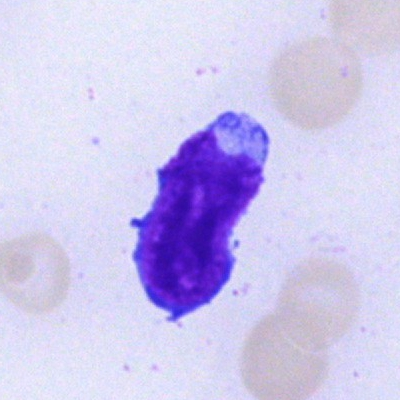
\includegraphics[width = 0.13\textwidth]{pics/Ergebnisse/orig1}}
\quad
\subfloat[Original 2]{
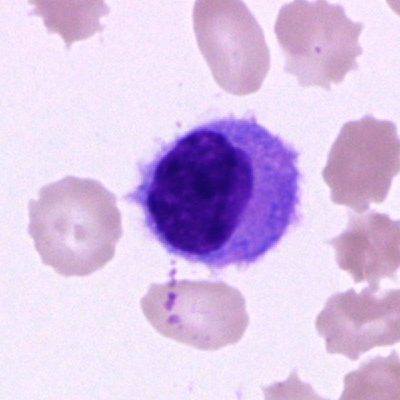
\includegraphics[width = 0.13\textwidth]{pics/Ergebnisse/orig4}}
\quad
\subfloat[Original 3]{
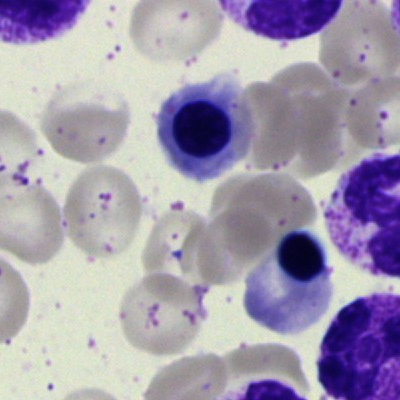
\includegraphics[width = 0.13\textwidth]{pics/Ergebnisse/orig2}}
\quad
\subfloat[Original 4]{
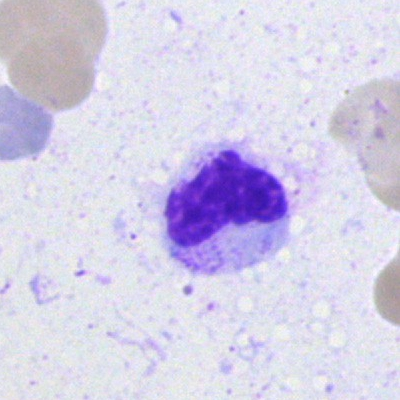
\includegraphics[width = 0.13\textwidth]{pics/Ergebnisse/orig3}}
\quad
\subfloat[Original 5]{
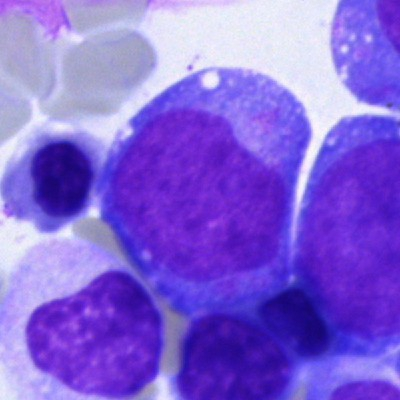
\includegraphics[width = 0.13\textwidth]{pics/Ergebnisse/orig5}}
\quad
\subfloat[Original 6]{
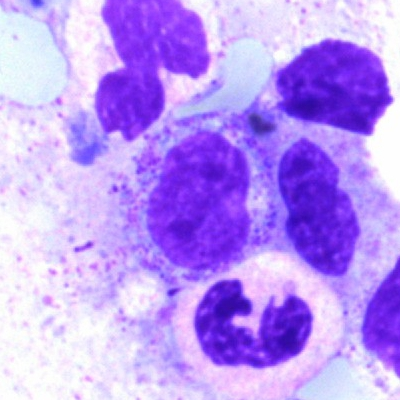
\includegraphics[width = 0.13\textwidth]{pics/Ergebnisse/orig6}}
\quad
\subfloat[Cluster 1]{
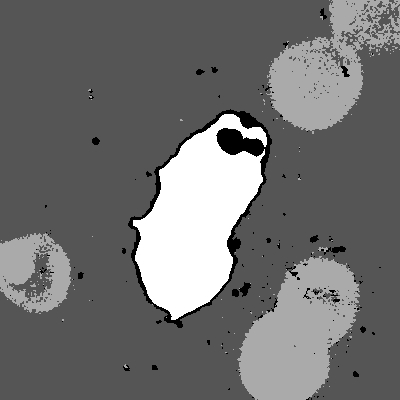
\includegraphics[width = 0.13\textwidth]{pics/Ergebnisse/cluster1}}
\quad
\subfloat[Cluster 2]{
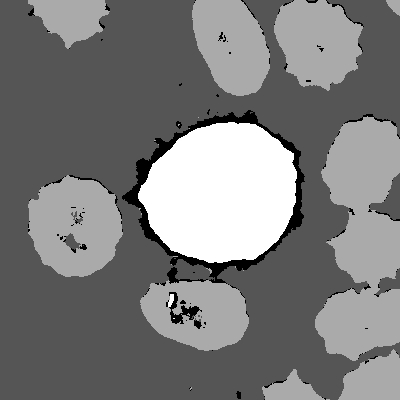
\includegraphics[width = 0.13\textwidth]{pics/Ergebnisse/cluster4}}
\quad
\subfloat[Cluster 3]{
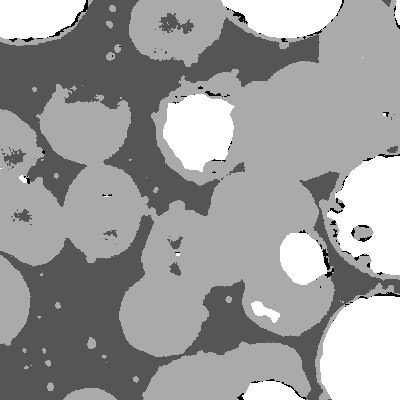
\includegraphics[width = 0.13\textwidth]{pics/Ergebnisse/cluster2}}
\quad
\subfloat[Cluster 4]{
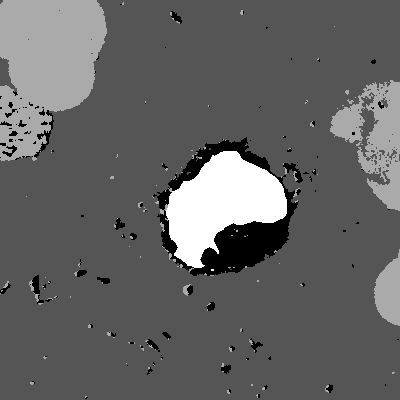
\includegraphics[width = 0.13\textwidth]{pics/Ergebnisse/cluster3}}
\quad
\subfloat[Cluster 5]{
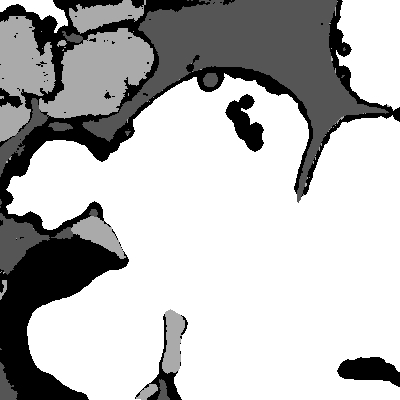
\includegraphics[width = 0.13\textwidth]{pics/Ergebnisse/cluster5}}
\quad
\subfloat[Cluster 6]{
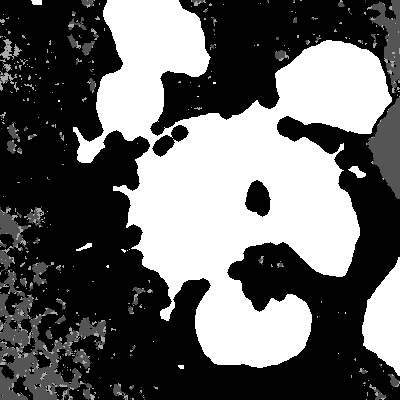
\includegraphics[width = 0.13\textwidth]{pics/Ergebnisse/cluster6}}
\caption[Beispiele Clusteralgorithmus]{Die Abbildung zeigt sechs Originalbilder in der ersten Zeile und die zugeh�rigen Ergebnisse des Clusteringverfahrens in der zweiten Zeile. In den ersten beiden F�llen zeigen sich sehr gute Ergebnisse, w�hrend die anderen vier kleinere und gr��ere Probleme aufzeigen. Bei den Clustern gilt folgende Zuordnung: wei� = gef�rbt, helles Grau = Sonstiges, dunkles Grau Hintergrund, schwarz = keine Information\label{fig:res_clustering}}
\end{figure} 

\section{Stainberechnung durch Optimierung}
Eine Beurteilung der Qualit�t der Stainvektoren f�r Color Deconvolution ist schwierig, da es keine echten Kriterien gibt. Zwar sagt z.B. \citeeig{landini2016}, dass der dritte Kanal m�glichst wei� sein soll, jedoch muss f�r diese Aussage unbedingt eine Hintergrundkorrektur durchgef�hrt werden. Vor allem bei sehr intensiv gef�rbten Zellkernen ist es jedoch auch mit Korrektur nicht m�glich, diese F�rbung nur durch zwei Komponenten auszudr�cken. Die zus�tzliche Information muss dann durch den dritten Kanal abgedeckt werden. Im vorliegenden Workflow gilt jedoch die Voraussetzung, dass sich die berechneten Vektoren f�r die einzelnen Bilder nur in geringem Ma� unterscheiden. Dies liegt an der Natur des Problems, da die verwendeten Farbstoffe f�r die verschiedenen Bilder gleich bleiben. Die getestete Idee die Vektoren mittels eines Optimierers zu berechnen konnte die Voraussetzung nicht erf�llen. Zwei verschiedene Beispiele wie die Zerlegung nach der Optimierung aussieht, sind in Abb. \ref{fig:stain_opt} zu sehen. 
\begin{figure}
\subfloat[Original 1]{
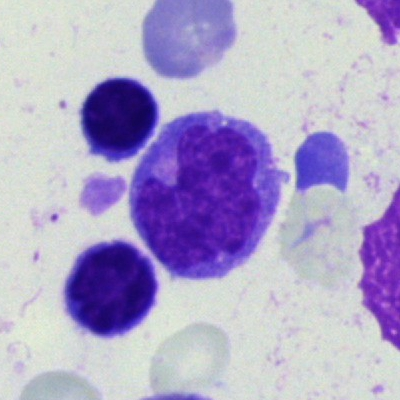
\includegraphics[width = 0.22\textwidth]{pics/Ergebnisse/opt_orig1}}
\quad
\subfloat[Kanal 1]{
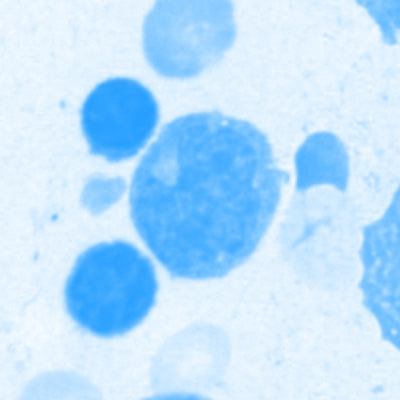
\includegraphics[width = 0.22\textwidth]{pics/Ergebnisse/opt_1_ch1}}
\quad
\subfloat[Kanal 2]{
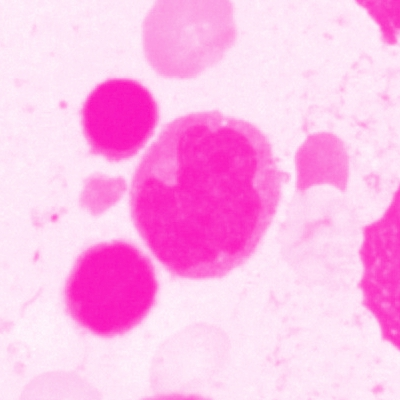
\includegraphics[width = 0.22\textwidth]{pics/Ergebnisse/opt_1_ch2}}
\quad
\subfloat[Kanal 3]{

\includegraphics[width = 0.22\textwidth]{pics/Ergebnisse/opt_1_ch3}}
\quad
\subfloat[Original 2]{
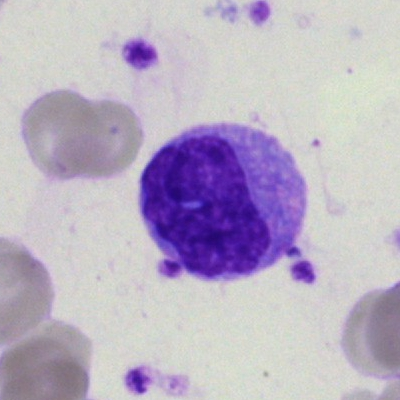
\includegraphics[width = 0.22\textwidth]{pics/Ergebnisse/opt_orig2}}
\quad
\subfloat[Kanal 1]{
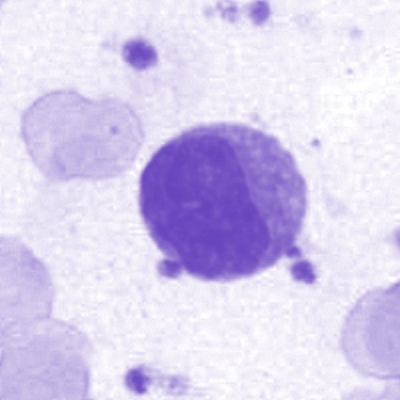
\includegraphics[width = 0.22\textwidth]{pics/Ergebnisse/opt_2_ch1}}
\quad
\subfloat[Kanal 2]{
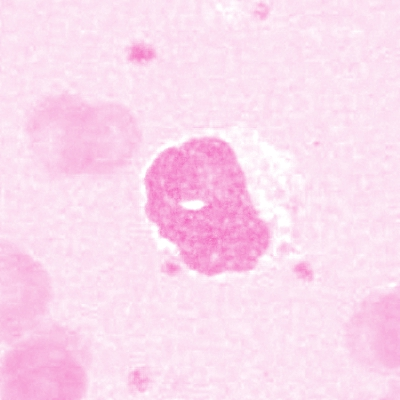
\includegraphics[width = 0.22\textwidth]{pics/Ergebnisse/opt_2_ch2}}
\quad
\subfloat[Kanal 3]{

\includegraphics[width = 0.22\textwidth]{pics/Ergebnisse/opt_2_ch3}}
\caption[Beispiele Color Deconvolution mit Optimierer]{Die obere Zeile zeig ein Beispiel, in welchem die Stainvektoren sich stark unterscheiden. In der unteren Zeile sind sich diese dagegen �hnlicher, was zu der deutlicheren Trennung zwischen Plasma und Kern f�hrt.\label{fig:stain_opt}} 
\end{figure}

\section{Vergleich der Korrelation in den einzelnen Farbr�umen}\label{sec:correlation}
\citeeig{reinhard2001color} f�hren eine Farbraumtransformation in den $l\alpha\beta$-Raum durch in welchem die eigentliche Anpassung stattfindet. Als Argumentation hierf�r dient die hohe Unabh�ngigkeit der einzelnen Kan�le, welche durch den Korrelationskoeffizienten messbar ist. Aus Tabelle \ref{tab:correlation} ist erkennbar, dass f�r die vorliegenden Daten die Kan�le $l$ und $\alpha$ eine starke Abh�ngigkeit aufweisen w�hrend $\beta$ sich von beiden stark unterscheidet. F�hrt man die Color Deconvolution mit den Stains von \citeeig{landini2016} durch, so existieren keine zwei Kan�le mit einer �hnlich hohen Abh�ngigkeit wie im $l\alpha\beta$-Raum, allerdings gibt es keinen Kanal, der stark von den anderen abweicht. Die Color Deconvolution nach Macenko liefert dagegen die beste Entkopplung der einzelnen Kan�le, was sich in den verh�ltnism��ig geringen Werten der Korrelationskoeffizienten zwischen allen Kan�len niederschl�gt. Im RGB-Farbraum weicht vor allem der Blaukanal von den anderen beiden ab, w�hrend R und G relativ stark korrelieren. 
\begin{table}[h]
\center
\caption[Korrelation in verschiedenen Farbr�umen]{Die Tabelle vergleicht die Korrelationskoeffizienten in verschiedenen Farbr�umen nach Transformation von Knochenmarkbildern. CD steht dabei f�r Color Deconvolution, Giemsa bzw. Macenko sind die jeweils verwendeten Stains.\label{tab:correlation}} 
\begin{tabular}{|c|c|c|c|c|}
\hline 
 & $\mathbf{l\alpha\beta}$ & \textbf{CD: Giemsa} & \textbf{CD: Macenko} & \textbf{RGB} \\ 
\hline 
\textbf{Kanal 1 und 2} & 0.9683 & 0.8555 & 0.3485 &  0.9078\\ 
\hline 
\textbf{Kanal 1 und 3} & 0.4453 & 0.7497 & 0.4321 & 0.7949 \\ 
\hline 
\textbf{Kanal 2 und 3} & 0.4750 & 0.8101 & 0.4174 & 0.6990 \\ 
\hline
\end{tabular}  
\end{table}

\section{Segmentierung}
\begin{figure}
\center
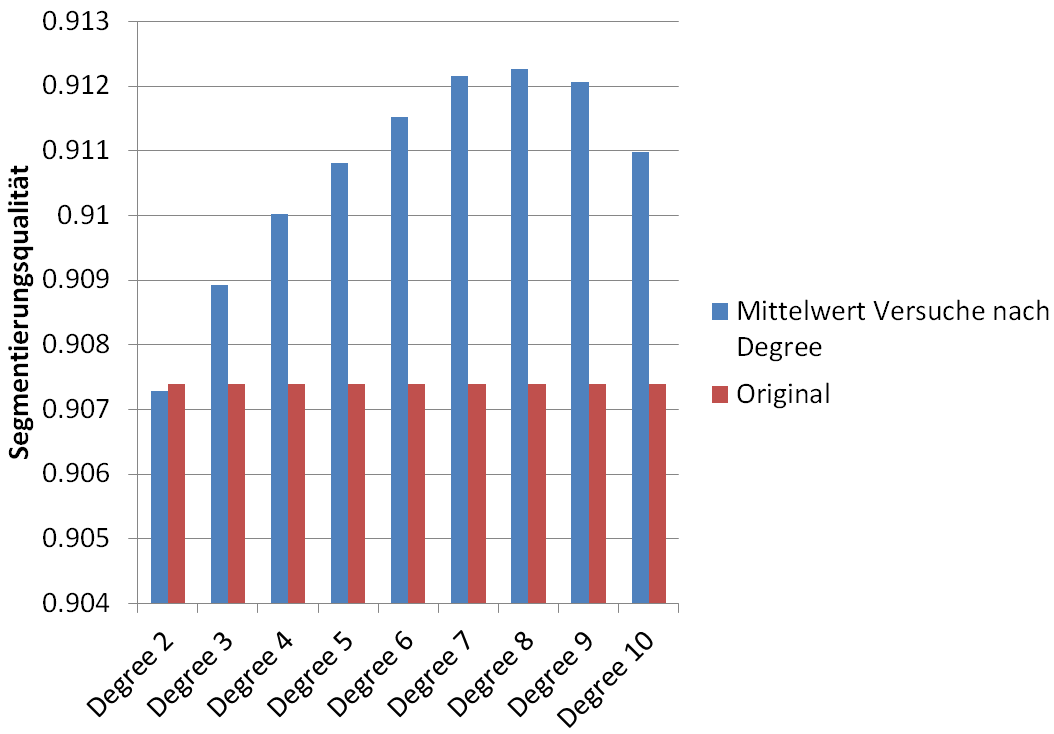
\includegraphics[width = 1.0\textwidth]{pics/Ergebnisse/NachDegreeImg_zelle}
\caption{Unterscheidung Segmentierung ganze Zelle nach Grad des B-Spline}
\end{figure}

\begin{figure}
\center
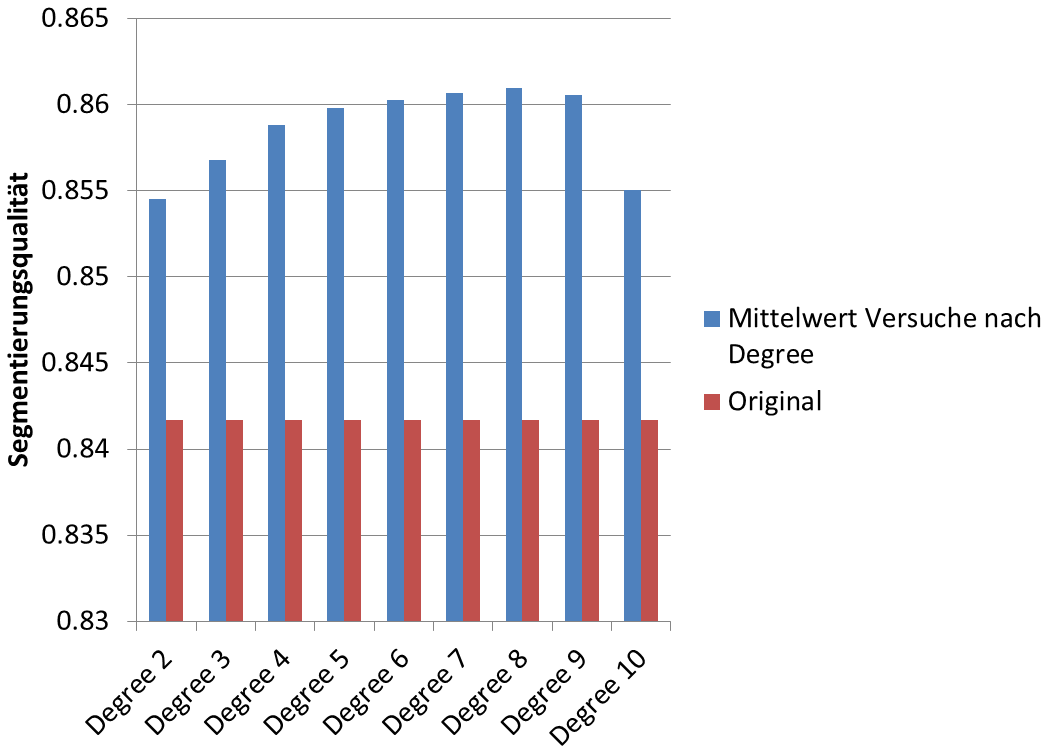
\includegraphics[width = 1.0\textwidth]{pics/Ergebnisse/NachDegreeImg_kern}
\caption{Unterscheidung Segmentierung Zellkern nach Grad des B-Spline}
\end{figure}

\begin{figure}
\center
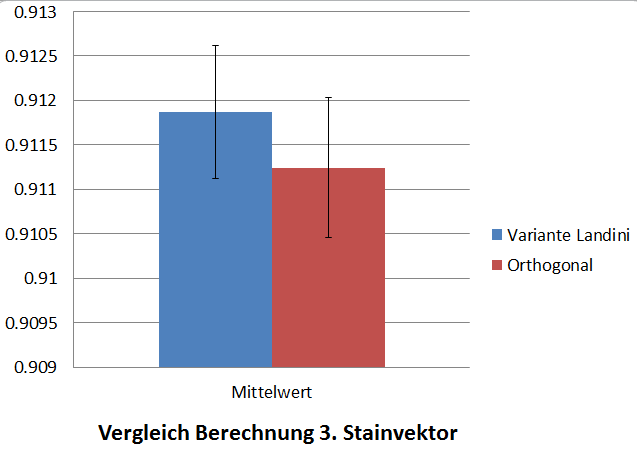
\includegraphics[width = 0.6\textwidth]{pics/Ergebnisse/Vergleich_ansatz_3vektor}
\caption[Vergleich Ans�tze Berechnung 3. Stainvektor]{Das Diagramm vergleicht die beiden implementierten Methoden zur Berechnung des 3. Stainvektors. Gezeigt ist jeweils der Mittelwert aus zw�lf unterschiedlichen Parameterkombinationen und die Standardabweichung.}
\end{figure}


\section{Klassifikation}


\chapter[Diskussion]{Diskussion}\label{sec:diskussion}
Im Folgenden werden die Ergebnisse aus Kapitel \ref{sec:ergebnis} diskutiert und bewertet. Dabei wird zun�chst allgemein auf die Ans�tze Farbnormalisierung eingegangen, im Anschluss werden die beiden Bereiche Segmentierung und Klassifikation behandelt. 

\section{Allgemein}\label{sec:dis_allgemein}
Vergleicht man den Farbeindruck f�r die verschiedenen getesteten Methoden, wird deutlich, dass Farbinformationen unterschiedlich stark verf�lscht werden. Dies soll in Abbildung \ref{fig:farbvergleich_norm} anhand von drei Beispielen verdeutlicht werden. Am deutlichsten ist dies bei Reinhard und bei der Anpassung von Mittelwert und Standardabweichung, welche sich nur im ge�nderten Farbraum unterscheiden. Als Zielbild diente dabei jeweils Referenzbild 1 (siehe Anhang \ref{app:reference}). Das Ergebnis ist dabei besonders stark durch den Anteil an gef�rbten Bereichen beeinflusst, was ein gro�er Nachteil der Verfahren ist. Weniger unnat�rlich wirken die Bilder nach Normalisierung mittels B-Spline und auf ein festgelegtes Pseudomaximum. Letztere Variante �hnelt im Hintergrund stark dem Original, da der dritte Kanal nicht angepasst wurde. Die gef�rbten Teile wirken insgesamt dunkler als beim Original, da das Maximum jeweils erh�ht wurde. Die mittels B-Splines angepassten Bilder normalisieren den Hintergrund sehr gut, so dass dieser sich in den verschiedenen Bildern stark �hnelt. Bei den gef�rbten Bereichen �ndert sich in Plasmabereichen teilweise das Verh�ltnis der beiden Farbstoffe. Zu sehen ist dieser Effekt beim Vergleich der Abbildungen \ref{fig:orig2} und \ref{fig:spline_giemsa2}. Bei der Zelle im Zentrum ist das Plasma nach der Anpassung leicht violett, w�hrend es zuvor bl�ulich erscheint. Die Referenz f�r beide F�lle ist Set 5 (siehe Anhang \ref{app:reference}), da hier die besten Ergebnisse f�r Segmentierung und Klassifikation erreicht werden wurden. 

\newcommand{\mywidth}{0.13}
\begin{figure}[htb]
\center
\subfloat[Original 1]{
\includegraphics[width = \mywidth\textwidth]{pics/Anhang/B/02_or}}
\quad
\subfloat[B-Spline Giemsa 1]{
\includegraphics[width = \mywidth\textwidth]{pics/Anhang/B/02_gie}}
\quad
\subfloat[B-Spline Macenko 1]{
\includegraphics[width = \mywidth\textwidth]{pics/Anhang/B/02_mac}}
\quad
\subfloat[Festes Maximum 1]{
\includegraphics[width = \mywidth\textwidth]{pics/Anhang/B/02_fix}}
\quad
\subfloat[Mean/Std 1]{
\includegraphics[width = \mywidth\textwidth]{pics/Anhang/B/02_std}}
\quad
\subfloat[Reinhard 1]{
\includegraphics[width = \mywidth\textwidth]{pics/Anhang/B/02_rei}}
\quad
\subfloat[Original 2]{
\includegraphics[width = \mywidth\textwidth]{pics/Anhang/B/03_or}\label{fig:orig2}}
\quad
\subfloat[B-Spline Giemsa 2]{
\includegraphics[width = \mywidth\textwidth]{pics/Anhang/B/03_gie}\label{fig:spline_giemsa2}}
\quad
\subfloat[B-Spline Macenko 2]{
\includegraphics[width = \mywidth\textwidth]{pics/Anhang/B/03_mac}}
\quad
\subfloat[Festes Maximum 2]{
\includegraphics[width = \mywidth\textwidth]{pics/Anhang/B/03_fix}}
\quad
\subfloat[Mean/Std 2]{
\includegraphics[width = \mywidth\textwidth]{pics/Anhang/B/03_std}}
\quad
\subfloat[Reinhard 2]{
\includegraphics[width = \mywidth\textwidth]{pics/Anhang/B/03_rei}}
\quad
\subfloat[Original 3]{
\includegraphics[width = \mywidth\textwidth]{pics/Anhang/B/13_or}}
\quad
\subfloat[B-Spline Giemsa 3]{
\includegraphics[width = \mywidth\textwidth]{pics/Anhang/B/13_gie}}
\quad
\subfloat[B-Spline Macenko 3]{
\includegraphics[width = \mywidth\textwidth]{pics/Anhang/B/13_mac}}
\quad
\subfloat[Festes Maximum 3]{
\includegraphics[width = \mywidth\textwidth]{pics/Anhang/B/13_fix}}
\quad
\subfloat[Mean/Std 3]{
\includegraphics[width = \mywidth\textwidth]{pics/Anhang/B/13_std}}
\quad
\subfloat[Reinhard 3]{
\includegraphics[width = \mywidth\textwidth]{pics/Anhang/B/13_rei}}
\caption[Vergleich Ausgabebilder unterschiedlicher Methoden]{Die Abbildung zeigt drei Beispiele, wie sich die Normalisierung durch verschiedene Methoden auf Originalbilder auswirkt.\label{fig:farbvergleich_norm} }
\end{figure}

Der Grund f�r die gr��te Stabilit�t der Anpassung mittels B-Splines liegt in der Ber�cksichtigung der verschiedenartigen Bereiche im Bild. Prinzipiell w�re dies auch f�r die anderen Methoden m�glich, jedoch w�rde dies bedeuten, dass die �quivalenten Regionen separat aneinander angepasst werden m�ssten. F�r das vorliegende Problem ist dies jedoch nicht m�glich, da die dadurch entstehenden Kanten, das Ergebnis des Segmentierungsalgorithmus vorweg nehmen w�rde. Bei der Anpassung durch einen B-Spline mit hohem Grad werden Kanten nicht unnat�rlich ver�ndert, da der B-Spline in hohem Ma�e stetig ist. Dadurch haben sich �hnelnde Pixel auch nach der Anpassung �hnliche Werte. Wird dagegen ein niedriger Grad gew�hlt, so haben eventuelle Ausrei�er ein starkes Gewicht. Im schlimmsten Fall kann dies dazu f�hren, dass der B-Spline nicht mehr monoton steigt. Ein Pixel der zuvor einen h�heren Wert hatte als ein anderer, k�nnte nach der Normalisierung eine niedrigere Intensit�t haben. Da sich Eingangsbild und Referenz stark unterscheiden k�nnen, was zu Ausrei�ern bei den Kontrollpunkten f�hrt, muss ein hoher Grad gew�hlt werden um die Stabilit�t der Ergebnisse zu gew�hrleisten. 
 
\section{Segmentierung}\label{sec:dis_seg}
Bei Betrachtung der Ergebnisse der Segmentierung ist festzustellen, dass die Normalisierung f�r die meisten Zellen keinen Unterschied macht. Liegen beispielsweise mehrere Zellen dicht aufeinander, so dass keine deutliche Grenze mehr erkennbar ist, so kann dieser Effekt durch die Anpassung nicht korrigiert werden. Sind dagegen alle Bereiche gut voneinander separierbar, so ist dies ebenfalls unabh�ngig von der Normalisierung und die automatische Segmentierung funktioniert f�r alle F�lle. Interessant sind die F�lle in der eine klare Verbesserung oder Verschlechterung vorliegt. Die Ergebnisse legen nahe, dass eine positive Ver�nderung deutlich h�ufiger ist als eine negative. F�r die Anpassung mittels B-Splines und auch beim festen Maximum gilt, dass die Farben dazu tendieren dunkler zu werden. Zwar wird auch der Hintergrund etwas dunkler, jedoch wird eine leichte F�rbung eliminiert, welche sich nachteilig auf die Segmentierung auswirken kann. F�r eine gute Trennung zwischen Plasma und Kern ist es optimal, wenn beide Regionen m�glichst homogen sind und sich gleichzeitig voneinander abgrenzen lassen. Werden als Referenz Bilder gew�hlt, bei denen der gef�rbte Bereich diese Eigenschaften erf�llt, so k�nnen diese auch auf die anzupassenden Bilder �bertragen werden. Die Abbildung \ref{fig:all_bspline} zeigt deutlich, dass nicht jedes Bild als Referenz geeignet ist, obwohl die automatische Segmentierung dort gut funktioniert. Es k�nnte z.B. sein, dass sich eine andere Zelle im Bild negativ auswirkt, oder st�rende Artefakte enthalten sind. In der vorliegenden Arbeit konnte eine Optimierung der Ergebnisse durch die Entfernung schwacher Einzelbilder aus dem Referenzset erzielt werden. Ein gewisse Vielfalt ist trotzdem notwendig um die Eigenschaften m�glichst vieler Zellen abzubilden. Mit Set 6, welches nur drei Zellen enth�lt (siehe Anhang \ref{app:reference}), wurden die Ergebnisse wieder leicht schlechter. Dass auch die Skalierung auf ein festes Maximum gute Ergebnisse bez�glich der Segmentierung erzielt, ist zu erwarten, da der Kontrast durch die Wahl eines verh�ltnism��ig hohem Maximum in den meisten F�llen erh�ht wurde. Eine Homogenisierung innerhalb Zellkern bzw. Plasma ist indes durch eine reine Skalierung nicht zu erreichen, was der Grund daf�r sein k�nnte, dass B-Splines f�r die Kernsegmentierung etwas besser funktionieren. 
Die Art einer Zelle ist von entscheidender Bedeutung f�r die automatische Segmentierung, sowie die Ver�nderung, welche mit einer m�glichen Anpassung einhergeht. Bei Normoblasten ist beispielsweise das Plasma relativ hell, was sie allgemein zu schwierigen F�llen f�r das Erkennen der ganzen Zelle macht. Nach Farbnormalisierung wird dieses Ergebnis durchschnittlich sogar noch etwas schlechter, weil im Clustering das Plasma h�ufig keiner Klasse zugeordnet werden kann. Dies hat zur Folge, dass sich stattdessen der Kontrast im Zellkern erh�ht. Daneben wird das Plasma noch heller und kann der Zelle nicht mehr zugeordnet werden. Durch den sehr dunklen Kern entspricht auch die Skalierung auf ein relativ hohes Pseudomaximum trotzdem einer Stauchung, wodurch das Plasma ebenfalls nochmals heller wird. Wird die ganze Zelle schon im Clustering-Schritt als gef�rbt erkannt, so besteht eine gute Chance, dass sowohl Zellkern- als auch Plasma sich gut voneinander und vom Hintergrund absetzen. Gerade die Segmentierung des Zellkerns hat durch die angewandten Normalisierungsverfahren im Mittel verbessert werden k�nnen.

\section{Klassifikation}\label{sec:dis_klass}

F�r die Klassifikation wurde eine verh�ltnism��ig kleine, jedoch repr�sentative Datenbank von 1000 Trainings- und 100 Testbildern eingesetzt. Dies hat zur Folge, dass die Ergebnisse nicht mit jenen verglichen werden k�nnen die \citeeig{krappe2016automated} erzielt haben, da dort mit �ber 140000 Zellen gearbeitet wurde. Aufgrund der geringen Zahl an Bildern in dieser Arbeit k�nnen hier nur Trends abgeleitet werden, die noch best�tigt werden m�ssen. Eine valide Aussage ist jedoch, dass die Qualit�t der Klassifikation mit besserer Segmentierung steigt. Dieser Zusammenhang ist in Abbildung \ref{fig:seg_vs_class} dargestellt, in der die Segmentierung bez�glich Zellkern mit der Trefferquote und der Genauigkeit der Experimente in Verbindung gebracht ist. Bei den beiden Ma�en f�r die Klassifikation sind  jeweils die Toleranzfelder ber�cksichtigt. Das Experiment mit der Handsegmentierung ist nicht mit einbezogen, da eine perfekte Qualit�t von 1.0 das Bild zu sehr beeinflussen und die restlichen Werte �berlagern w�rde. Die jeweils steigenden Trendlinien zeigen, dass eine verbesserte Trefferquote jeweils nicht zu lasten der Genauigkeit geht.

\begin{figure}
\center
\subfloat[Trefferquote]{
\includegraphics[width = 0.47\textwidth]{pics/Diskussion/seg_vs_class}}
\quad
\subfloat[Genauigkeit]{
\includegraphics[width = 0.47\textwidth]{pics/Diskussion/seg_vs_class_precision}}
\caption[Klassifikation in Abh�ngigkeit von der Segmentierung]{Abbildung \textbf{(a)} zeigt die Trefferwahrscheinlichkeit der Klassifikationsexperimente in Abh�ngigkeit von der Qualit�t der verwendeten Segmentierung. \textbf{(b)} �quivalent dazu die Genauigkeit in Abh�ngigkeit der Segmentierun. In blau sind dabei die Datenpunkte zu sehen, von denen jeder f�r ein Experiment steht. In schwarz ist jeweils die zugeh�rige lineare Trendlinie zu sehen.\label{fig:seg_vs_class}}
\end{figure}

Der Einfluss der Ver�nderung der Farbeeigenschaften der Zelle, kann nicht eindeutig bewertet werden. Die Experimente 1 und 10, in denen die gleiche automatische Segmentierung mit normalisierten bzw. originalen Bildern getestet wurde, lieferten vor allem unter Ber�cksichtigung der Toleranzfelder sehr �hnliche Resultate. Die Bef�rchtung, dass eine Anpassung aller verschiedenen Zellarten auf die gleichen Farbeigenschaften sich nachteilig auf die Klassifikationsf�higkeit auswirken k�nnte hat sich jedoch nicht best�tigt. Falls ein Trend in den vorliegenden Experimenten vorhanden ist, so ist er durch den Einfluss der Segmentierung �berlagert.  

\chapter[Zusammenfassung und Ausblick]{Zusammenfassung und Ausblick}\label{sec:ausblick}
W�hrend der Bearbeitung der vorliegenden Arbeit haben sich Erkenntnisse und Ideen ergeben, welche in der Zukunft eingearbeitet werden k�nnen. Diese sollen in den folgenden Abschnitten vorgestellt werden. Zun�chst wird die Arbeit jedoch kurz zusammengefasst.

\section{Zusammenfassung}
In der vorliegenden Arbeit wurden verschiedene Methoden zur Farbnormalisierung getestet und in Bezug auf die Auswirkung auf Segmentierung und Klassifikation bewertet. Das Standardverfahren nach Reinhard f�hrt die Anpassung einzeln in den Kan�len des sogenannten $l\alpha\beta$-Raum durch, in welchem die Kan�le m�glichst stark korrelieren. Dem gegen�bergestellt wurden Verfahren, welche auf Color Deconvolution basieren. Diese Farbraumtransformation hat f�r die vorliegende Anwendung den Vorteil, dass sie die Informationen �ber verwendete Farbstoffe aufgreift. Die Anpassung der so getrennten Kan�le erfolgte mittels B-Splines, einer Skalierung der Histogramme und der �bertragung von Mittelwert und Standardabweichung. Grundlage f�r die Color Deconvolution ist die Definition der Stainvektoren. Hierf�r wurden eine von \citeeig{macenko2009method} eingef�hrte automatische Methode sowie eigene Ideen, die auf der Definition eines Optimierungsproblems basieren, umgesetzt. Automatische Methoden sind fehleranf�llig solange sie nur auf kleinen Bildausschnitten arbeiten, weshalb die manuelle Bestimmung am sichersten ist. Bei der Segmentierung zeigten sich leichte Verbesserungen f�r die Betrachtung der ganzen Zelle, deutlicher war diese f�r die Trennung zwischen Kern und Plasma. F�r die meisten Zellen blieben die Segmentierungsqualit�t in einem �hnlichen Bereich, Ausrei�er waren jedoch h�ufiger verbessert als verschlechtert. Die Resultate der Klassifikation legen nahe, dass vor allem die genauere Segmentierung einen positiven Einfluss hat und die Ergebnisse dadurch verbessert werden k�nnen. Inwieweit die Klassifikation durch die Ver�nderung der Farbeigenschaften beeinflusst wird, konnte aufgrund einer relativ kleinen Trainings- und Testdatenbank nicht abschlie�end gekl�rt werden. 

\section{Verwendung gr��erer Bildausschnitte}
Die quantitative Auswertung der Farbnormalisierung erfolgte in dieser Arbeit auf relativ kleinen Ausschnitten von 400$\times$400 Pixeln. Die Ursache lag dabei in einer fehlenden Grundwahrheit f�r die vorhandenen Ausschnitte mit einer Gr��e von 2452$\times$2056 Pixeln. Wie schon im vorhergehenden Kapitel \ref{sec:dis_klass} angemerkt, ist es problematisch die Farbeigenschaften von verschiedenartigen Zellen aufeinander abzubilden. Dieser Effekt kann mit der Verwendung gr��erer Bilder zumindest reduziert werden, da sowohl f�r Eingangs- als auch Referenzbild eine gr��ere Zahl Zellen vorhanden ist. Die Daten basieren auf dem ersten Teil des von \citeeig{krappe2014lokalisierung} verwendeten Segmentierungsverfahren, in welchem die Zellen lokalisiert werden \cite{krappe2014lokalisierung}. Aus diesem Grund wurde in der vorliegenden Arbeit die Ver�nderung f�r den zweiten Teil analysiert. Die Ergebnisse legen nahe, dass ein positiver Einfluss von Farbnormalisierungsverfahren auch f�r den ersten Schritt m�glich ist. Dies muss in der Zukunft jedoch noch nachgewiesen werden. In Anhang \ref{app:big} sind Beispiele f�r die Anpassung mittels B-Splines auf gro�en Daten gezeigt.

\section{Segmentierungsalgorithmus}
Eine Color Deconvolution mit geeigneten Stainvektoren k�nnte dazu eingesetzt werden die automatische Segmentierung zu verbessern. Die durch das Verfahren von Macenko gefundenen Stains f�hren bei bestimmten Zellarten zu einer Aufteilung von Plasma und Kern in unterschiedliche Kan�le. In einem Grauwertbild, welches auf dem Verh�ltnis der Intensit�ten dieser Kan�le basiert, sind die beiden Bereiche gut identifizierbar. Auch der Gradient innerhalb der Kan�le muss jedoch beachtet werden, da es Zellarten gibt, bei denen Zellkern und -plasma die gleiche Farbe haben, jedoch mit unterschiedlichen Intensit�ten. Bei diesen Zellen bleibt das Verh�ltnis der Kan�le gleich. Die geringe Korrelation zwischen den einzelnen Kan�len nach dieser Farbraumtransformation, welche in Abschnitt \ref{sec:correlation} nachgewiesen wurde, hat in jedem Fall das Potential, die Trennung zwischen Kern und Plasma zu verbessern. 

\section{Klassifikation}
Anhand der Klassifikationsresultate dieser Arbeit k�nnen noch keine validen Aussagen dar�ber getroffen werden, inwieweit die Farbver�nderungen der einzelnen Zellen das Ergebnis beeinflussen (siehe Abschnitt \ref{sec:dis_klass}). Aus diesem Grund ist ein Test mit vergr��erter Datenbank unerl�sslich. Sollte sich eine Verbesserung der Klassifikationsergebnisse nur aufgrund der genaueren Segmentierung ergeben, die Farb�nderungen jedoch einen negativen Einfluss auf die Klassifikation haben, kann die neue Segmentierung mit den Originalbildern verbunden werden. Sowohl angepasste als auch unver�nderte Farbbilder sind in der Prozesskette verf�gbar, so dass zur Optimierung ein Austausch der Informationen m�glich ist. 
%\include{chapters/Zusammenfasung}


% ---------- Anhang ----------
% Die Datei Appendix.tex wird automatisch erzeugt!

%\begin{appendix}
%\input{appendices/Anhang}
%\end{appendix}

% ----------------------------

% Erzeugt das Literaturverzeichnis
%\bibliographystyle{plain}
%\bibliography{Literatur}
\newpage
\phantomsection \label{bibliography}
\addcontentsline{toc}{chapter}{Literaturverzeichnis} 
\bibliographystyle{plainnat} %numbers, order: alphabetical
%\bibliographystyle{natdin} %numbers, order: alphabetical
\bibliography{bib/quellen}

% Erzeugt eine Seite mit der Erklaerung
\declaration{nutzung}

\end{document}
